\documentclass[
	article,
	12pt,				% tamanho da fonte
	oneside,
	a4paper,			% tamanho do papel. 
	% -- opções da classe abntex2 --
	%chapter=TITLE,		% títulos de capítulos convertidos em letras maiúsculas
	%section=TITLE,		% títulos de seções convertidos em letras maiúsculas
	%subsection=TITLE,	% títulos de subseções convertidos em letras maiúsculas
	%subsubsection=TITLE,% títulos de subsubseções convertidos em letras maiúsculas
	% -- opções do pacote babel --
	english,			% idioma adicional para hifenização
	brazil				% o último idioma é o principal do documento
	]{abntex2}

% ---
% Pacotes básicos 
% ---
\usepackage{lmodern}			% Usa a fonte Latin Modern			
\usepackage[T1]{fontenc}		% Selecao de codigos de fonte.
\usepackage[utf8]{inputenc}		% Codificacao do documento (conversão automática dos acentos)
\usepackage{lastpage}			% Usado pela Ficha catalográfica
\usepackage{indentfirst}		% Indenta o primeiro parágrafo de cada seção.
\usepackage{color}				% Controle das cores
\usepackage{graphicx}			% Inclusão de gráficos
\usepackage{microtype} 			% para melhorias de justificação
\usepackage{float}
% ---

% ---
% Pacotes de citações
% ---
\usepackage[brazilian,hyperpageref]{backref}	 % Paginas com as citações na bibl
\usepackage[alf,abnt-emphasize=bf]{abntex2cite}	% Citações padrão ABNT
\let\tt\ttfamily

% --- 
% CONFIGURAÇÕES DE PACOTES
% --- 

% ---
% Configurações do pacote backref
% Usado sem a opção hyperpageref de backref
\renewcommand{\backrefpagesname}{Citado na(s) página(s):~}
% Texto padrão antes do número das páginas
\renewcommand{\backref}{}
% Define os textos da citação
\renewcommand*{\backrefalt}[4]{
	\ifcase #1 %
		Nenhuma citação no texto.%
	\or
		Citado na página #2.%
	\else
		Citado #1 vezes nas páginas #2.%
	\fi}%
% ---
\graphicspath{{./media}}

% ---
% Informações de dados para CAPA e FOLHA DE ROSTO
% ---
\titulo{NOVADMIN: Módulo de Orçamento para Sistema ERP}
\autor{
	Matheus Tomazella\\
	Rafael Cesar Vanzo\\
	Samuel dos Santos Carneiro\\
}
\local{Americana -- SP}
\data{2026}
\orientador{Leonardo Grando}
\instituicao{
	CENTRO UNIVERSITÁRIO SALESIANO DE SÃO PAULO
	\par
	UNISAL -- CAMPUS MARIA AUXILIADORA
}
\tipotrabalho{Trabalho de Conclusão de Curso (TCC)}
% O preambulo deve conter o tipo do trabalho, o objetivo, 
% o nome da instituição e a área de concentração 
\preambulo{Trabalho de Conclusão de Curso apresentado como exigência parcial para a obtenção do grau de Bacharel em Engenharia da Computação no Centro Universitário Salesiano de São Paulo.\\
Orientador: Prof. Dr. Leonardo Grando.}
% ---


% ---
% Configurações de aparência do PDF final

% alterando o aspecto da cor azul
\definecolor{blue}{RGB}{41,5,195}

% informações do PDF
\makeatletter
\hypersetup{
     	%pagebackref=true,
		pdftitle={\@title}, 
		pdfauthor={\@author},
    	pdfsubject={\imprimirpreambulo},
	    pdfcreator={LaTeX with abnTeX2},
		pdfkeywords={ERP, Orçamento, Arquitetura de Software}, 
		colorlinks=true,       		% false: boxed links; true: colored links
    	linkcolor=blue,          	% color of internal links
    	citecolor=blue,        		% color of links to bibliography
    	filecolor=magenta,      		% color of file links
		urlcolor=blue,
		bookmarksdepth=4
}
\makeatother
% --- 

% --- 
% Espaçamentos entre linhas e parágrafos 
% --- 

% O tamanho do parágrafo é dado por:
\setlength{\parindent}{1.3cm}

\renewcommand{\thesection}{\arabic{section}}
\renewcommand{\thesubsection}{\thesection.\arabic{subsection}}
\renewcommand{\thesubsubsection}{\thesubsection.\arabic{subsubsection}}

\makeevenhead{abntheadings}{\thepage}{}{}
\makeoddhead{abntheadings}{}{}{\thepage}

\renewcommand{\ABNTEXchapterfontsize}{\normalsize}
\renewcommand{\ABNTEXsectionfontsize}{\normalsize}
\renewcommand{\ABNTEXsubsectionfontsize}{\normalsize}
\renewcommand{\ABNTEXsubsubsectionfontsize}{\normalsize}
\renewcommand{\ABNTEXfontereduzida}{\normalsize}
\renewcommand{\ABNTEXchapterfont}{\rmfamily}
\renewcommand{\ABNTEXpartfont}{\rmfamily}
\renewcommand{\ABNTEXsectionfont}{\rmfamily}
\renewcommand{\ABNTEXsubsectionfont}{\rmfamily\bfseries}
\renewcommand{\ABNTEXsubsubsectionfont}{\rmfamily\bfseries}
\renewcommand{\ABNTEXsubsubsubsectionfont}{\rmfamily}
\renewcommand{\chaptitlefont}{\rmfamily\bfseries\normalsize}
\renewcommand{\cftsubsectionfont}{\rmfamily\bfseries}
\renewcommand{\cftsubsectionpagefont}{\rmfamily\bfseries}
\renewcommand{\cftsubsubsectionfont}{\rmfamily\bfseries}
\renewcommand{\cftsubsubsectionpagefont}{\rmfamily\bfseries}
\makeatletter
\renewcommand{\contentsname}{SUMÁRIO}
\renewcommand{\listadesiglasname}{\textbf{LISTA DE ABREVIATURAS E SIGLAS}}
\renewcommand{\tableofcontents}{%
  \chapter*{\bfseries\MakeUppercase{\contentsname}}%
  \@mkboth{\MakeUppercase{\contentsname}}{\MakeUppercase{\contentsname}}%
  \@starttoc{toc}%
}
\makeatother

\makeatletter
\renewcommand{\section}{% 
  \@startsection{section}{1}{\z@}%
    {-3.5ex \@plus -1ex \@minus -.2ex}%
    {2.3ex \@plus.2ex}%
    {\normalfont\rmfamily\bfseries\MakeUppercase}%
}
\renewcommand{\subsection}{%
  \@startsection{subsection}{2}{\z@}%
    {-3.25ex\@plus -1ex \@minus -.2ex}%
    {1.5ex\@plus .2ex}%
    {\normalfont\rmfamily\bfseries}%
}
\makeatother

% ---
% compila o indice
% ---
\makeindex
\makeglossary
\renewcommand{\glossitem}[4]{#1 -- #2\newline\par}
\renewcommand{\glossaryspace}{\par}
% ---

% ----
% Início do documento
% ----
\begin{document}
\renewcommand{\bibname}{\textbf{REFERÊNCIAS}}
\renewcommand{\glossaryname}{GLOSSÁRIO}

% Retira espaço extra obsoleto entre as frases.
\frenchspacing

% ----------------------------------------------------------
% ELEMENTOS PRÉ-TEXTUAIS
% ----------------------------------------------------------
% \pretextual

% ---
% Capa
% ---
\begin{capa}
	\centering
	\imprimirinstituicao\\

	\vspace*{1cm}

	\ABNTEXchapterfontsize{\imprimirautor}

	\vspace*{4.5cm}

	\ABNTEXchapterfontsize{\rmfamily\bfseries\imprimirtitulo}

	\vfill

	\imprimirlocal\\
	\imprimirdata

	\vspace{3cm}
\end{capa}
% ---

% ---
% Folha de rosto
% ---
\begin{folhaderosto}
	\centering
	\ABNTEXchapterfontsize{\imprimirautor}

	\vspace*{4.5cm}

	\ABNTEXchapterfontsize{\rmfamily\bfseries\imprimirtitulo}

	\vspace{1.5cm}

	\noindent\hspace*{8cm}%
	\begin{minipage}{\dimexpr\textwidth-8cm\relax}
		\raggedright
		\imprimirpreambulo
	\end{minipage}

	\vfill

	\imprimirlocal\\
	\imprimirdata

	\vspace{3cm}
\end{folhaderosto}
\clearpage
% ---

% ---
% Folha de aprovação
% ---
\begin{folhadeaprovacao}
	\begingroup\centering
	\ABNTEXchapterfontsize{\imprimirautor}

	\vspace*{1.5cm}

	\ABNTEXchapterfontsize{\rmfamily\bfseries\imprimirtitulo}

	\vspace{1.5cm}

	\noindent\hspace*{8cm}%
	\begin{minipage}{\dimexpr\textwidth-8cm\relax}
		\raggedright
		\imprimirpreambulo
	\end{minipage}

	\vspace{1.5cm}
	\endgroup

	Trabalho de Conclusão de Curso defendido e aprovado em \_\_/11/2026, pela
	comissão julgadora:

	\centering

	\vspace{1.5cm}
	\rule{12cm}{0.4pt}\par
	Prof. Dr. Leonardo Grando, UNISAL\\

	% \vspace{1.5cm}
	% \rule{12cm}{0.4pt}\par
	% Prof. Me. Loren, Ipsum\\

	\vfill

	\imprimirlocal\\
	\imprimirdata

	\vspace{3cm}
\end{folhadeaprovacao}
\clearpage
% ---

% ---
% RESUMOS
% ---

% resumo em português
\setlength{\absparsep}{18pt} % ajusta o espaçamento dos parágrafos do resumo
\begin{resumo}[\textbf{RESUMO}]
	\indent
	Apresenta a implementação de um módulo de orçamento, construído com o objetivo de centralizar dados relevantes e automatizar etapas de cálculo e a geração do documento de proposta, reduzindo o esforço necessário e aumentando a consistência do processo.
	O módulo foi desenvolvido com uma arquitetura em camadas, utilizando React para a interface web, Node.js com TypeScript e Express.js para a API REST, e PostgreSQL para o armazenamento de dados em um processo iterativo e incremental, com ênfase na validação contínua junto aos usuários finais e na entrega progressiva de funcionalidades.
	A interface organiza o processo de orçamentação em etapas sequenciais, facilitando o trabalho do usuário e garantindo flexibilidade para atender a situações reais do domínio.
	O resultado é um sistema que espelha fielmente o fluxo de trabalho da empresa, incorporando suas nomenclaturas, etapas e regras de negócio específicas, eliminando a necessidade de adequações operacionais forçadas.

	Palavras-chave: arquitetura de software; orçamento; ERP.
\end{resumo}
\clearpage

% resumo em inglês
\begin{resumo}[\textbf{ABSTRACT}]
	\begin{otherlanguage*}{english}
		\indent
		Presents the implementation of a module for quotes, built to centralize relevant data and automate calculation steps and the generation of the proposal document, reducing the necessary effort and increasing the consistency of the process.
		The module was developed with a layered architecture, using React for the web interface, Node.js with TypeScript and Express.js for the REST API, and PostgreSQL for data storage in an iterative and incremental process, with emphasis on continuous validation with end users and progressive delivery of features.
		The interface organizes the quoting process into sequential steps, facilitating the user's work and ensuring flexibility to meet real-world situations in the domain.
		The result is a system that faithfully mirrors the company's workflow, incorporating its nomenclature, steps, and specific business rules, eliminating the need for forced operational adjustments.

		Key-words: software architecture; quoting; ERP.
	\end{otherlanguage*}
\end{resumo}
\clearpage
% ---

% ---
% inserir lista de ilustrações
% ---
% \pdfbookmark[0]{\listfigurename}{lof}
% \listoffigures*
% \cleardoublepage
% ---

% ---
% inserir lista de tabelas
% ---
% \pdfbookmark[0]{\listtablename}{lot}
% \listoftables*
% \cleardoublepage
% ---

% ---
% inserir lista de abreviaturas e siglas
% ---
% \begin{siglas}
% 	\item[API] Interface de Programação de Aplicações
% 	\item[CI/CD] Integração Contínua e Entrega Contínua
% 	\item[DOCX] Formato de arquivo do Microsoft Word baseado em XML
% 	\item[ERP] Planejamento de Recursos Empresariais (Enterprise Resource Planning)
% 	\item[HTML] Linguagem de Marcação de Hipertexto (HyperText Markup Language)
% 	\item[MER] Modelo Entidade-Relacionamento
% 	\item[PDF] Formato de Documento Portátil (Portable Document Format)
% 	\item[REST] Transferência de Estado Representacional (Representational State
% 	Transfer)
% 	\item[SQL] Linguagem de Consulta Estruturada (Structured Query Language)
% 	\item[TCC] Trabalho de Conclusão de Curso
% 	\item[UNISAL] Centro Universitário Salesiano de São Paulo
% \end{siglas}
% ---

% ---
% inserir o sumario
% ---
\pdfbookmark[0]{SUMÁRIO}{toc}
\tableofcontents
\cleardoublepage
% ---

% ----------------------------------------------------------
% ELEMENTOS TEXTUAIS
% ----------------------------------------------------------
\textual

% ----------------------------------------------------------
% Introdução (exemplo de capítulo sem numeração, mas presente no Sumário)
% ----------------------------------------------------------
\section{INTRODUÇÃO}
% ----------------------------------------------------------

O processo de elaboração de orçamentos constitui atividade recorrente em
empresas de engenharia e construção. Envolvendo a coleta e consolidação de
informações sobre clientes, obras, materiais e regras de precificação, é um
processo complexo que tem potenciais riscos significativos de inconsistência e
retrabalho, podendo gerar danos à reputação e ao lucro da empresa em casos
extremos.

Esse trabalho descreve a extensão de um sistema previamente construído com a
implementação de um módulo especializado para geração de orçamentos e propostas
de serviço. O objetivo geral é centralizar dados relevantes e automatizar
etapas de cálculo e a geração do documento de proposta, reduzindo o esforço
necessário e aumentando a consistência do processo.

A interface segue o molde do sistema previamente implantado, utilizando uma
plataforma web clara, com edição organizada em etapas sequenciais e suporte a
colaboração controlada quando aplicável.

\subsection{Contexto Empresarial}

O cliente é uma empresa especializada na fabricação de moldes reutilizáveis de
concreto para o setor de engenharia civil. Historicamente, o processo de
elaboração de propostas comerciais era executado por meio de planilhas
eletrônicas e procedimentos manuais, o que gerava riscos significativos de
inconsistência, dificuldade de rastreamento de decisões e reduzida capacidade
de automação.

Reconhecendo essas limitações operacionais, a empresa decidiu ampliar seu
sistema corporativo NOVADMIN (já em uso para outras funcionalidades) por meio
da implementação de um módulo especializado para orçamentação. Esta expansão
permite consolidar dados dispersos, automatizar etapas críticas e estabelecer
um ponto único de controle e auditoria para o processo de proposta.

Dessa forma, diferentemente de soluções de mercado que, por mais configuráveis
que sejam, impõem uma lógica genérica à qual a empresa precisa se adaptar, o
módulo de orçamentação do sistema espelha fielmente o fluxo de trabalho da
empresa, incorporando suas nomenclaturas, etapas e regras de negócio
específicas. Essa aderência ao processo interno elimina a necessidade de
adequações operacionais forçadas e garante que a ferramenta sirva à empresa, e
não o contrário.

\subsection{Objetivos}

Os principais objetivos deste projeto são: expandir o banco de dados para
suportar as entidades de fornecedor, material, orçamento, escopo, elemento,
custo fixo e opção de precificação; adicionar as funcionalidades necessárias
para gerenciar esses dados; automatizar o cálculo dos custos do serviço a
partir das informações inseridas; automatizar a geração do documento de
proposta de serviço; e implementar um sistema de versionamento para os
orçamentos. \glossary{Versionamento}{Processo de manter e rastrear múltiplas
	versões de um registro, preservando as relações entre elas para fins de
	auditoria e rastreabilidade.}

Além disso, os objetivos não funcionais incluem oferecer uma interface simples
e intuitiva, manter o estilo previamente estabelecido para o sistema, garantir
flexibilidade para que o usuário não seja limitado em suas operações, priorizar
a automação dos processos para reduzir a possibilidade de erro humano e
aumentar a eficiência do sistema, e permitir que múltiplos usuários editem
partes de um registro simultaneamente.

\section{DESENVOLVIMENTO}
Essa seção descreve a metodologia adotada para a implementação do projeto, o
fluxo de trabalho do usuário quando visto isolado da tecnologia e detalhes
sobre as decisões técnicas arquiteturais e de infraestrutura que foram tomadas
para atender aos requisitos do sistema.

\subsection{Metodologia}

O desenvolvimento do módulo foi baseado em \textit{frameworks} ágeis, seguindo
uma abordagem iterativa e incremental, com ênfase na validação contínua junto
aos usuários finais e na entrega progressiva de funcionalidades.

Os requisitos funcionais foram levantados por meio de sessões de trabalho com a
equipe operacional da empresa, garantindo que as necessidades reais do domínio
fossem compreendidas e incorporadas no \textit{design}. Durante as fases de
implementação, testes unitários foram aplicados sistematicamente para validar a
lógica de negócio, especialmente nas operações críticas de cálculo dos custos,
utilizando dados gerados pelas planilhas substituídas pelo sistema como
garantia de que os resultados continuariam condizentes com o processo.

Aspectos como a alta flexibilidade requerida pelo domínio do sistema (que
demanda suporte a múltiplas exceções de regras) e a necessidade de compreender
o contexto específico do cliente foram gerenciados por meio de ciclos de
avaliação contínua, permitindo refinar a solução conforme o aprendizado
progrediu.

A \autoref{fig:cronograma} apresenta o cronograma do projeto, que foi
organizado em etapas complementares. A fase inicial de \textit{design} teve
duração de um mês, seguida por cinco meses de desenvolvimento do
\textit{backend} e quatro meses de desenvolvimento do \textit{frontend}. O
trabalho escrito foi produzido em paralelo às etapas de desenvolvimento,
durante três meses. No dois meses finais, foram realizados simultaneamente os
testes e correções e o polimento do documento.

\begin{figure}[H]
	\caption{\label{fig:cronograma}Cronograma de desenvolvimento do projeto}
	\centering
	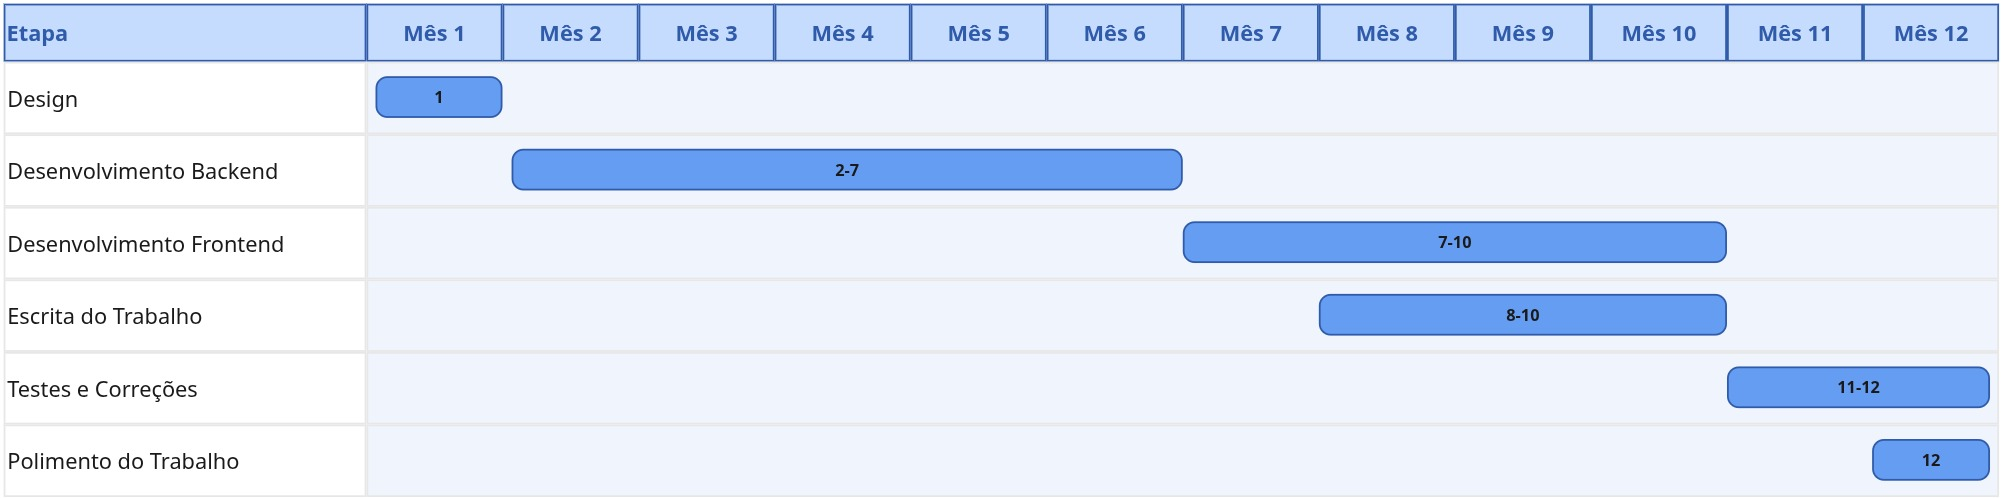
\includegraphics[width=\textwidth]{gantt.jpg}
	\legend{Fonte: Elaborado pelos autores, 2026.}
\end{figure}

\subsection{Fluxo de Trabalho do Usuário}\label{sec:fluxo}

Esta seção descreve o fluxo de trabalho do módulo de forma abstrata,
apresentando o caminho percorrido pelo usuário para elaborar um orçamento de
maneira isolada, ou seja, sem considerar detalhes de implementação, tecnologias
empregadas ou a aparência das telas. Esses aspectos são tratados nas seções
seguintes.

A \autoref{fig:fluxo} demonstra o fluxo completo, desde a inserção das
entidades que compõem o Orçamento até a exportação do documento da proposta.

\begin{figure}[H]
	\caption{\label{fig:fluxo}Diagrama de fluxo de trabalho do módulo de orçamento}
	\centering
	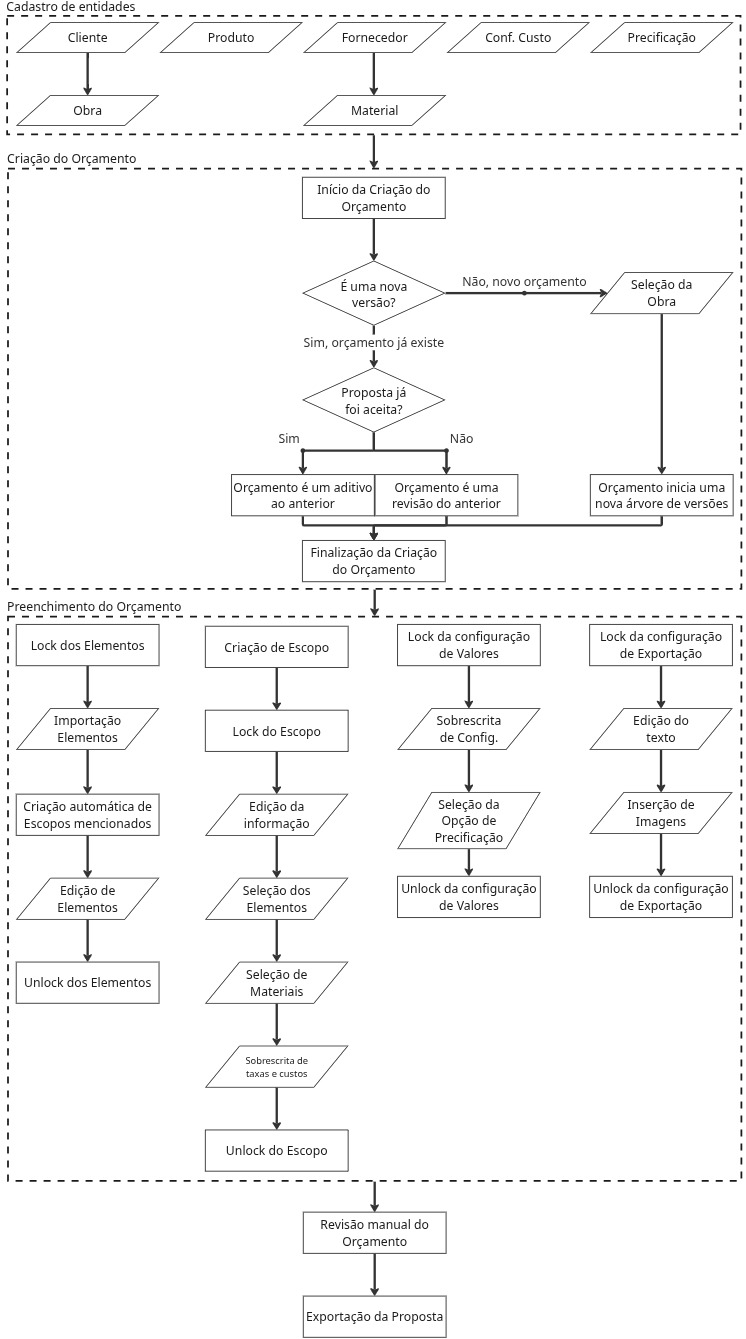
\includegraphics[width=\textwidth,height=0.90\textheight,keepaspectratio]{fluxo-novo.jpg}
	\legend{Fonte: Elaborado pelos autores, 2026.}
\end{figure}

O fluxo se inicia com a inserção das entidades que compõem o Orçamento:
Cliente, Obra, Produto, Fornecedor, Material, Custos Fixos e Opções de
Precificação. Todas são entidades simples, sem relacionamentos em sua
composição, exceto por Material, que deve ser associado a um Fornecedor e Obra
que deve ser associada a um Cliente.

Em seguida, o Orçamento é criado, sendo associado a um Cliente e a uma Obra,
podendo também ser uma nova versão de um Orçamento anterior. Uma nova versão
mantém relação com o Orçamento de origem e pode ser de dois tipos: uma revisão,
caso o Orçamento ainda esteja aberto, ou um aditivo, caso já tenha sido
concluído.

Posteriormente, ocorre a etapa de gerenciamento dos Elementos, na qual o
usuário pode realizar a importação por meio de arquivo, bem como efetuar
edições manuais. Durante esse processo, o gerenciamento de Elementos permanece
indisponível para outros usuários. A inserção de Elementos por um arquivo
também permite ao usuário criar automaticamente os Escopos correspondentes.

A seguir, pode ser feito o gerenciamento dos Escopos, uma entidade que
representa um trecho do projeto e contém Elementos e configurações. Aqui o
usuário também associa os materiais aos elementos e pode sobrescrever valores
de cálculo para o contexto do Escopo. A fim de evitar conflitos de edição, o
acesso a cada Escopo é restrito a um único usuário enquanto este estiver em
uso.

A etapa seguinte envolve o gerenciamento de configurações de precificação, como
sobrescrever valores de cálculo para o contexto do Orçamento, e selecionar a
opção de precificação que será utilizada para o cálculo do valor final.

Por fim, ocorre a configuração do documento, etapa que permite ao usuário
ajustar textos e formatação, inserir imagens e configurar a ordenação de
elementos. Aqui o usuário também deve conferir manualmente as informações e
valores finais calculados. Feito isso, a proposta pode ser exportada em formato
PDF ou DOCX, finalizando o processo.

Um elemento importante desse processo é a inclusão do sistema de sobrescrita de
valores para os escopos de cálculo. Configurações como a definição dos
produtos, preços de materiais e taxas de consumo de matéria-prima para
determinado tipo de elemento são realizadas fora de um orçamento e servem como
fonte geral, porém todas podem ser sobrescritas tanto para um determinado
Orçamento quanto para um Escopo naquele Orçamento.

Isso permite que o sistema se adapte a situações reais, que não necessariamente
seguem o fluxo padrão, mas ainda são de grande importância, como a aplicação de
descontos ou situações incomuns como falta de funcionários ou materiais. Essa
flexibilidade é um dos fatores que tornam o sistema um substituto real ao
processo anterior, garantindo que se adeque à empresa e não o contrário.

\subsection{Tecnologias e Infraestrutura}\label{sec:tecnologias}
O módulo de orçamento foi organizado em camadas para separar a interface, as
regras de negócio e a persistência dos dados. Essa divisão evita que a tela
dependa diretamente da forma como o banco está estruturado e facilita a
manutenção quando alguma parte do processo precisa ser ajustada.

A camada de apresentação consiste em uma interface web desenvolvida em React
\cite{react}, escolha realizada pela necessidade de uma navegação responsiva
entre listas, formulários e abas de edição, para a qual o React oferece
abstrações adequadas. Essa tecnologia também já era utilizada para o sistema já
implantado, permitindo uma integração simples.

A camada de lógica de negócios consiste em uma API (Application Programming
Interface) REST (Representational State Transfer) \cite{fielding2000}
implementada em Node.js \cite{nodejs} com TypeScript \cite{typescript} e
Express.js \cite{expressjs}. A API concentra as regras de domínio do módulo e
expõe operações de criação, leitura, atualização, remoção e bloqueio de
registros. A separação entre camadas foi adotada para reduzir acoplamento,
facilitar evolução independente e centralizar regras de negócio em um único
ponto de controle. \glossary{API}{Application Programming Interface. Interface
	que permite a comunicação entre dois sistemas de software.}
\glossary{REST}{Representational State Transfer. Estilo arquitetural para APIs
	que define restrições sobre como os serviços devem se comunicar via HTTP.}
\glossary{Node.js}{Ambiente de execução JavaScript no lado do servidor,
	utilizado para construção de APIs e aplicações de rede.}
\glossary{TypeScript}{Linguagem de programação baseada em JavaScript que
	adiciona tipagem ao código, aumentando a segurança e a previsibilidade do
	desenvolvimento.} \glossary{Express.js}{Framework web para Node.js utilizado
	para a construção de APIs e servidores HTTP.}

Uma decisão arquitetural relevante foi a utilização de uma biblioteca
compartilhada entre essas camadas, contendo regras de domínio e tipos de dados
relevantes. Essa abordagem reduz duplicação de código, principalmente em
cálculos, transformações de dados e tipos. Consequentemente, garante
uniformidade de comportamento entre as camadas e reduz a probabilidade de
divergências entre interface e processos internos.

Para armazenamento de dados foi adotado PostgreSQL \cite{postgresql}, um
sistema gerenciador relacional que oferece suporte adequado aos requisitos de
integridade referencial e transacional demandados pelo domínio. O modelo
relacional favorece a preservação de consistência e facilita consultas
agregadas sobre múltiplas entidades. \glossary{Transação}{Operação indivisível
	executada completamente ou revertida em sua totalidade (tudo ou nada),
	garantindo a integridade dos dados.}

A \autoref{fig:database} apresenta o esquema definido para atender às
necessidades do sistema, representado por meio de um diagrama MER (Modelo
Entidade-Relacionamento) \cite{chen1976entity}.

\begin{figure}[H]
	\caption{\label{fig:database}Diagrama MER do banco de dados}
	\centering
	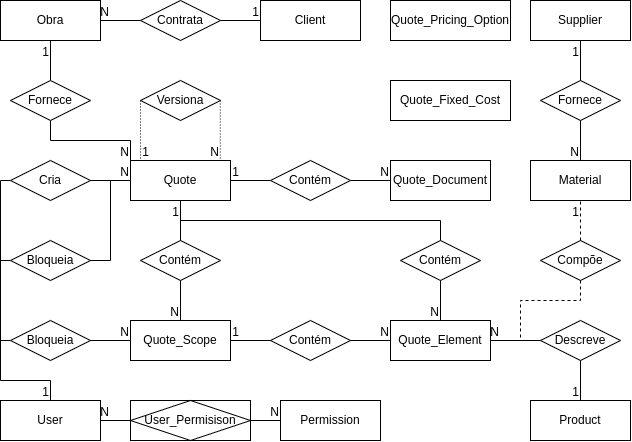
\includegraphics[width=\textwidth]{database.png}
	\legend{Fonte: Elaborado pelos autores, 2026.}
\end{figure}

A análise da estrutura começa pelas entidades que representam elementos mais
simples: clientes (\textit{Client}), produtos (\textit{Product}), obras,
fornecedores (\textit{Supplier}), materiais (\textit{Material}), usuários
(\textit{User}), opções de precificação (\textit{Quote\_Pricing\_Option}) e
custos fixos (\textit{Quote\_Fixed\_Cost}) que possuem poucas interações entre
si e no geral servem apenas para guardar dados que serão úteis para outros
elementos mais complexos.

Os elementos do orçamento são armazenados na tabela Quote\_Element, cujos
registros se relacionam com a tabela Quote\_Scope, responsável por armazenar
informações dos escopos do projeto, como dados de identificação e configuração.
Por sua vez, o escopo está associado à tabela Quote, que representa o
Orçamento.

A tabela Quote\_Document também se relaciona com o Orçamento e armazena os
anexos utilizados para a criação do documento de proposta, como imagens dos
projetos referenciados.

Adicionalmente, a tabela Permission armazena as permissões do sistema e se
relaciona com os usuários por meio da tabela intermediária User\_Permission,
sendo essencial para o controle de acesso.

Essa organização permite que o sistema trate suas entidades de forma
independente, facilitando a implementação de sistemas como o bloqueio de edição
necessário para a edição concorrente de itens em um mesmo Orçamento.

Assim, a arquitetura foi concebida para favorecer evolução incremental. Esta
abordagem reduz riscos técnicos e viabiliza entrega progressiva de
funcionalidades.

\subsubsection{Infraestrutura e Implantação}

Para facilitar desenvolvimento, testes e implantação, o projeto adota
contêineres Docker \cite{docker} e orquestração via Docker Compose
\cite{dockercompose}. A utilização de contêineres garante que o ambiente de
execução seja consistente entre máquinas de desenvolvimento e servidores de
produção, reduzindo inconsistências. A orquestração é empregada para montar
serviços dependentes (API, banco de dados, serviços complementares) com
configuração unificada, simplificando a criação de ambientes reproduzíveis e
isolados. \glossary{Docker}{Plataforma de conteinerização que permite empacotar
	aplicações e suas dependências em ambientes isolados e reproduzíveis chamados
	contêineres.} \glossary{Docker Compose}{Ferramenta complementar ao Docker que
	permite definir e orquestrar múltiplos contêineres com uma única configuração,
	simplificando a criação de ambientes complexos.} \glossary{CI/CD}{Continuous
	Integration/Continuous Delivery (Integração e Entrega Contínuas). Conjunto de
	práticas que automatizam a integração, teste e entrega de software ao longo do
	desenvolvimento.}

O projeto adota um banco de dados relacional (SQL) devido à natureza fortemente
relacional dos dados de domínio. O PostgreSQL foi selecionado pela robustez,
maturidade de funcionalidades, comunidade ativa e suporte adequado em ambientes
empresariais.

Para implantações em infraestrutura local, o projeto inclui scripts e
configurações de serviço que automatizam inicialização e parada do sistema com
integração ao estado do sistema operacional. Esta abordagem permite reinício
automático do serviço, diminuindo o tempo que fica indisponível.

Além disso, para reduzir risco em \textit{deploys} de produção, a
infraestrutura foi montada de forma a suportar um fluxo de \textit{release}
\textit{Blue/Green} \cite{fowler2010}. Nesse modelo, mantém-se dois ambientes
idênticos, porém enquanto um está ativo e disponível aos usuários o outro
recebe a nova versão, que é testada. Após validação, o roteamento é
redirecionado para o ambiente atualizado, permitindo uma recuperação rápida ao
manter a outra instância intacta caso algum problema ocorra. Com imagens Docker
e orquestração, esse padrão é de simples implementação e combina bem com
práticas de CI/CD para \textit{deploys} controlados.

A infraestrutura também prevê centralização de logs, monitoramento básico e
políticas de \textit{backup/restore} para o PostgreSQL em múltiplos locais. A
configuração por contêiner facilita a instrumentação e a padronização de
métricas e alertas e o armazenamento de versões antigas do banco de dados
garante recuperação em situações catastróficas com perda mínima de trabalho.

Por fim, o sistema implementa um modelo de controle de acesso baseado em
permissões, associando cada usuário a papéis que determinam quais
funcionalidades e dados são acessíveis. As permissões são gerenciáveis,
permitindo que administradores designem papéis conforme a estrutura
organizacional e responsabilidades de cada operador. Todas as operações
sensíveis (criação, alteração, remoção de orçamentos e escopos) são registradas
em logs de auditoria, permitindo rastreamento completo de quem fez o quê e
quando.

\subsection{Resultados}
\subsubsection{Interface do Usuário}\label{sec:interface}

A interface do módulo foi concebida para organizar o processo de orçamentação
em etapas sequenciais, reduzindo complexidade cognitiva e facilitando o
trabalho do usuário. A \autoref{fig:quote_list} demonstra a tela inicial, que
reúne as operações principais (pesquisa, filtros, criação), enquanto a edição é
realizada por meio de abas temáticas.

\begin{figure}[H]
	\caption{\label{fig:quote_list}Interface -- Listagem de Orçamentos}
	\centering
	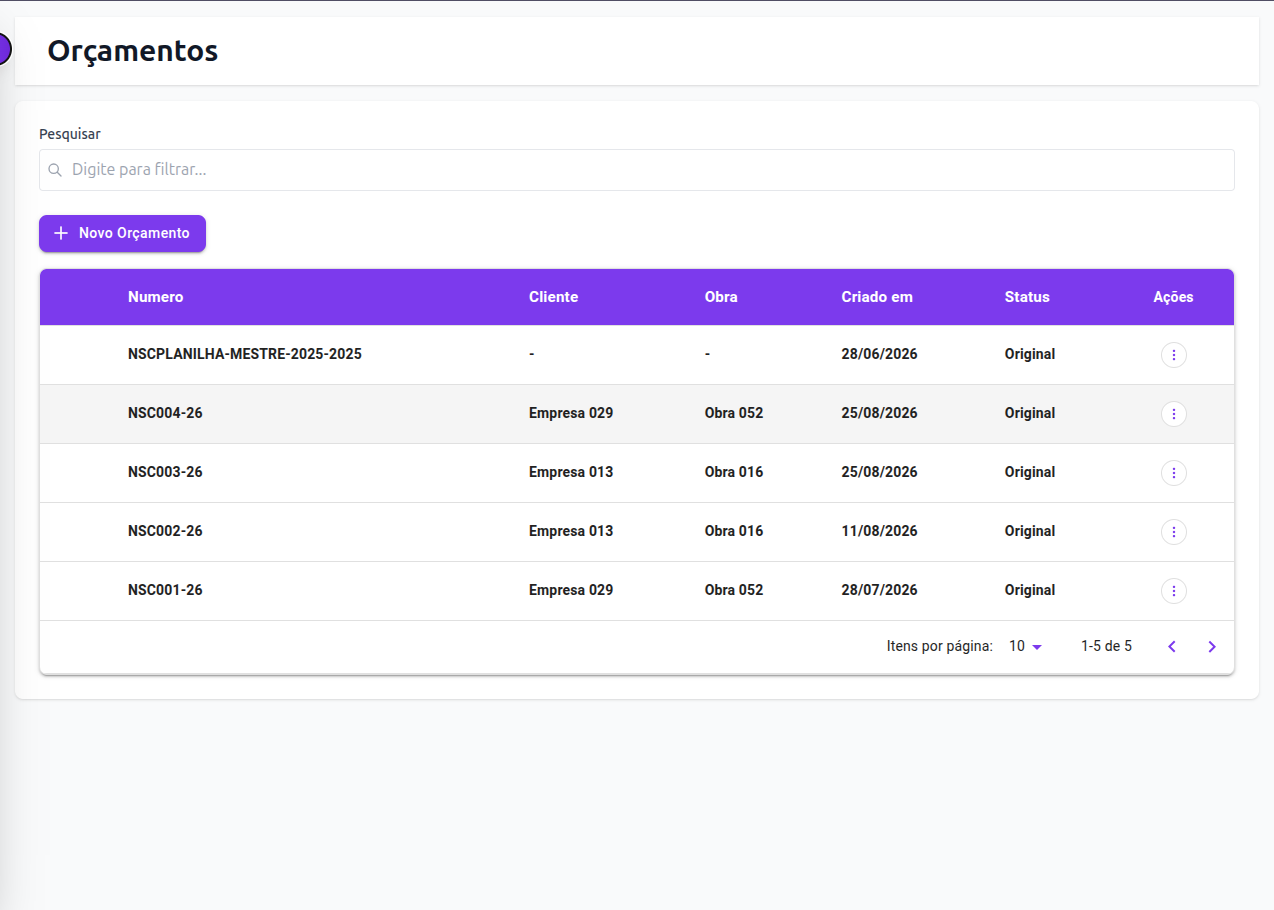
\includegraphics[width=\textwidth]{quote_list.png}
	\legend{Fonte: Elaborado pelos autores, 2026.}
\end{figure}

A \autoref{fig:elements} demonstra a aba Elementos, que permite o gerenciamento
da lista de elementos do orçamento, com suporte a importação por arquivo e
edição manual em lote. Sua interface inclui três seções para cada categoria de
elemento onde os itens são mostrados em um formato de tabela, incluindo apenas
os campos válidos para seu tipo.

\begin{figure}[H]
	\caption{\label{fig:elements}Interface -- Gerenciamento de Elementos}
	\centering
	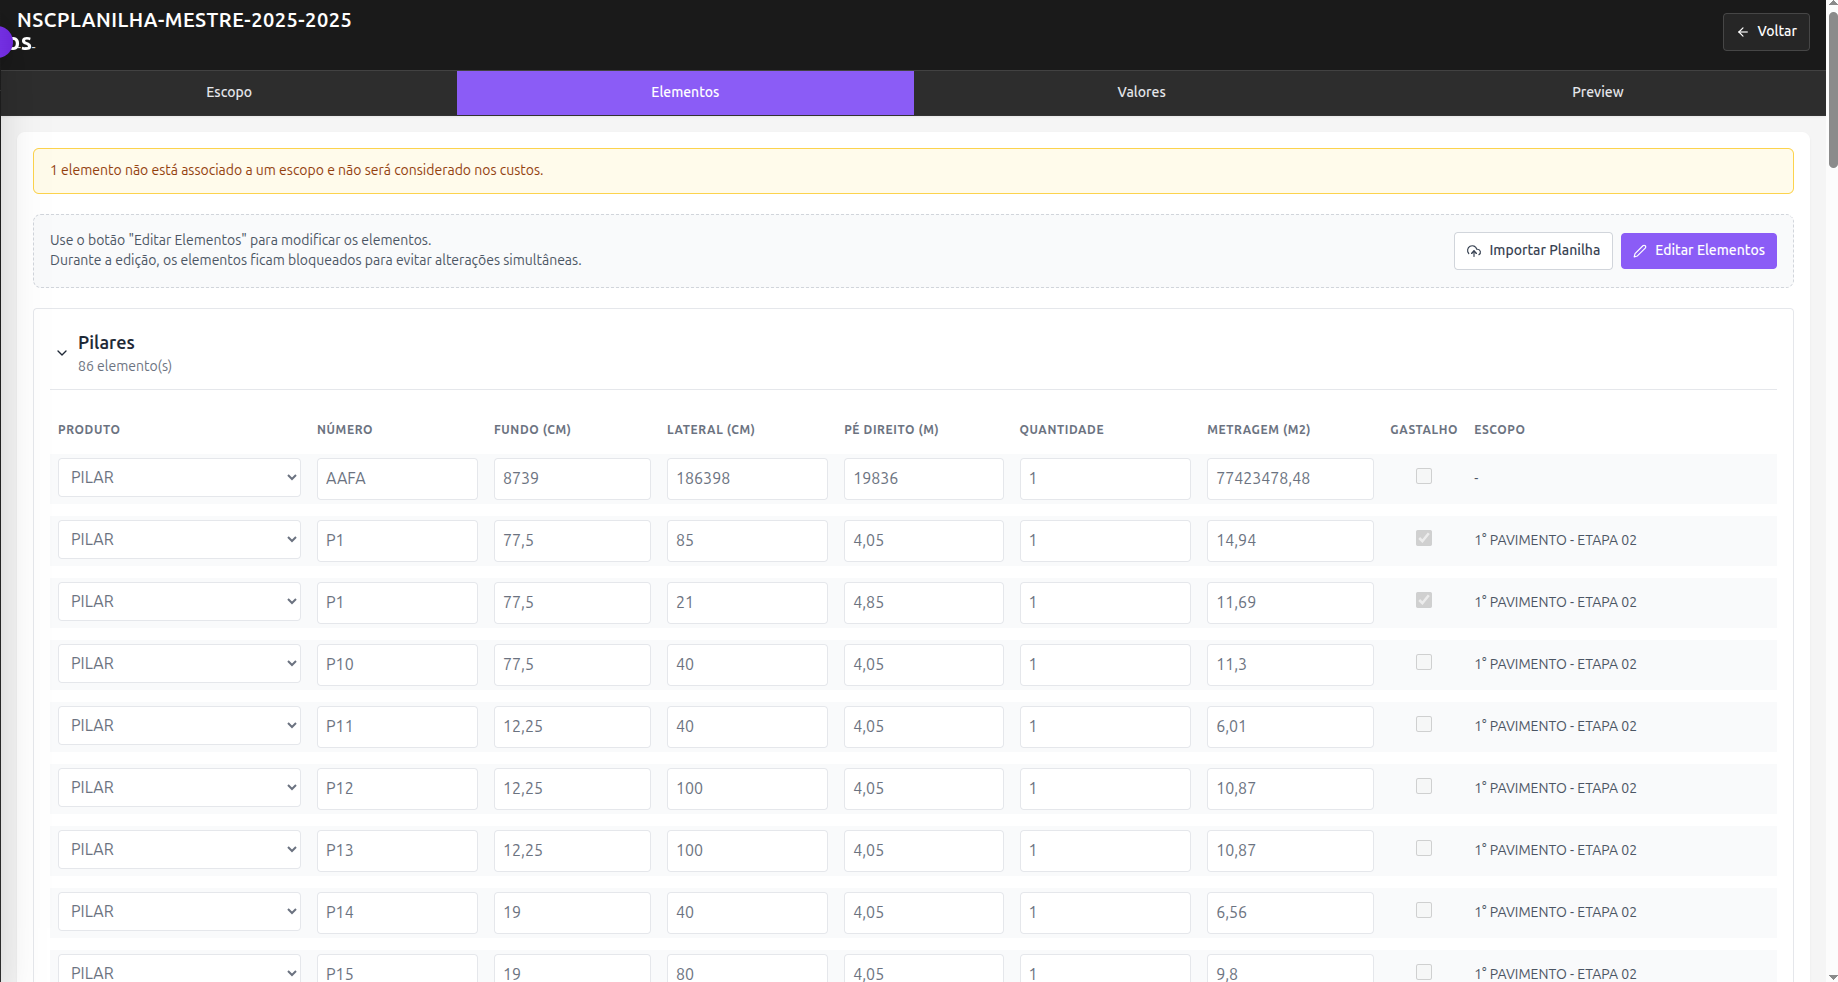
\includegraphics[width=\textwidth]{elements.png}
	\legend{Fonte: Elaborado pelos autores, 2026.}
\end{figure}

A utilização de seções colapsáveis permite ao usuário ver apenas o que precisa,
evitando a necessidade de rolar a tela por grandes distâncias, principalmente
quando essa seção pode incluir centenas de itens em cada categoria. Esse
elemento de \textit{design} é muito utilizado na criação desse sistema.

O botão “Editar Elementos” inclui uma explicação sobre o bloqueio de edição da
seção para outros usuários durante o uso. Essa inclusão é importante para
garantir que o usuário entenda a necessidade de limitar o tempo de uso e
principalmente para que não confunda a impossibilidade de editar os elementos
com um erro no sistema e possua as informações necessárias para liberar seu
acesso.

A \autoref{fig:scope_list} demonstra a aba Escopos, que separa os projetos em
partes menores, permitindo a delimitação de grupos de elementos que podem
possuir configurações diferentes. Cada Escopo inclui um resumo de suas
informações, incluindo tanto os itens simples, como nomes de responsáveis,
quanto uma tabela que resume os elementos inclusos. Isso permite ao usuário
extrair uma grande quantidade de informação sem a necessidade de analisar as
minúcias do Escopo.

\begin{figure}[H]
	\caption{\label{fig:scope_list}Interface -- Aba de listagem de Escopos}
	\centering
	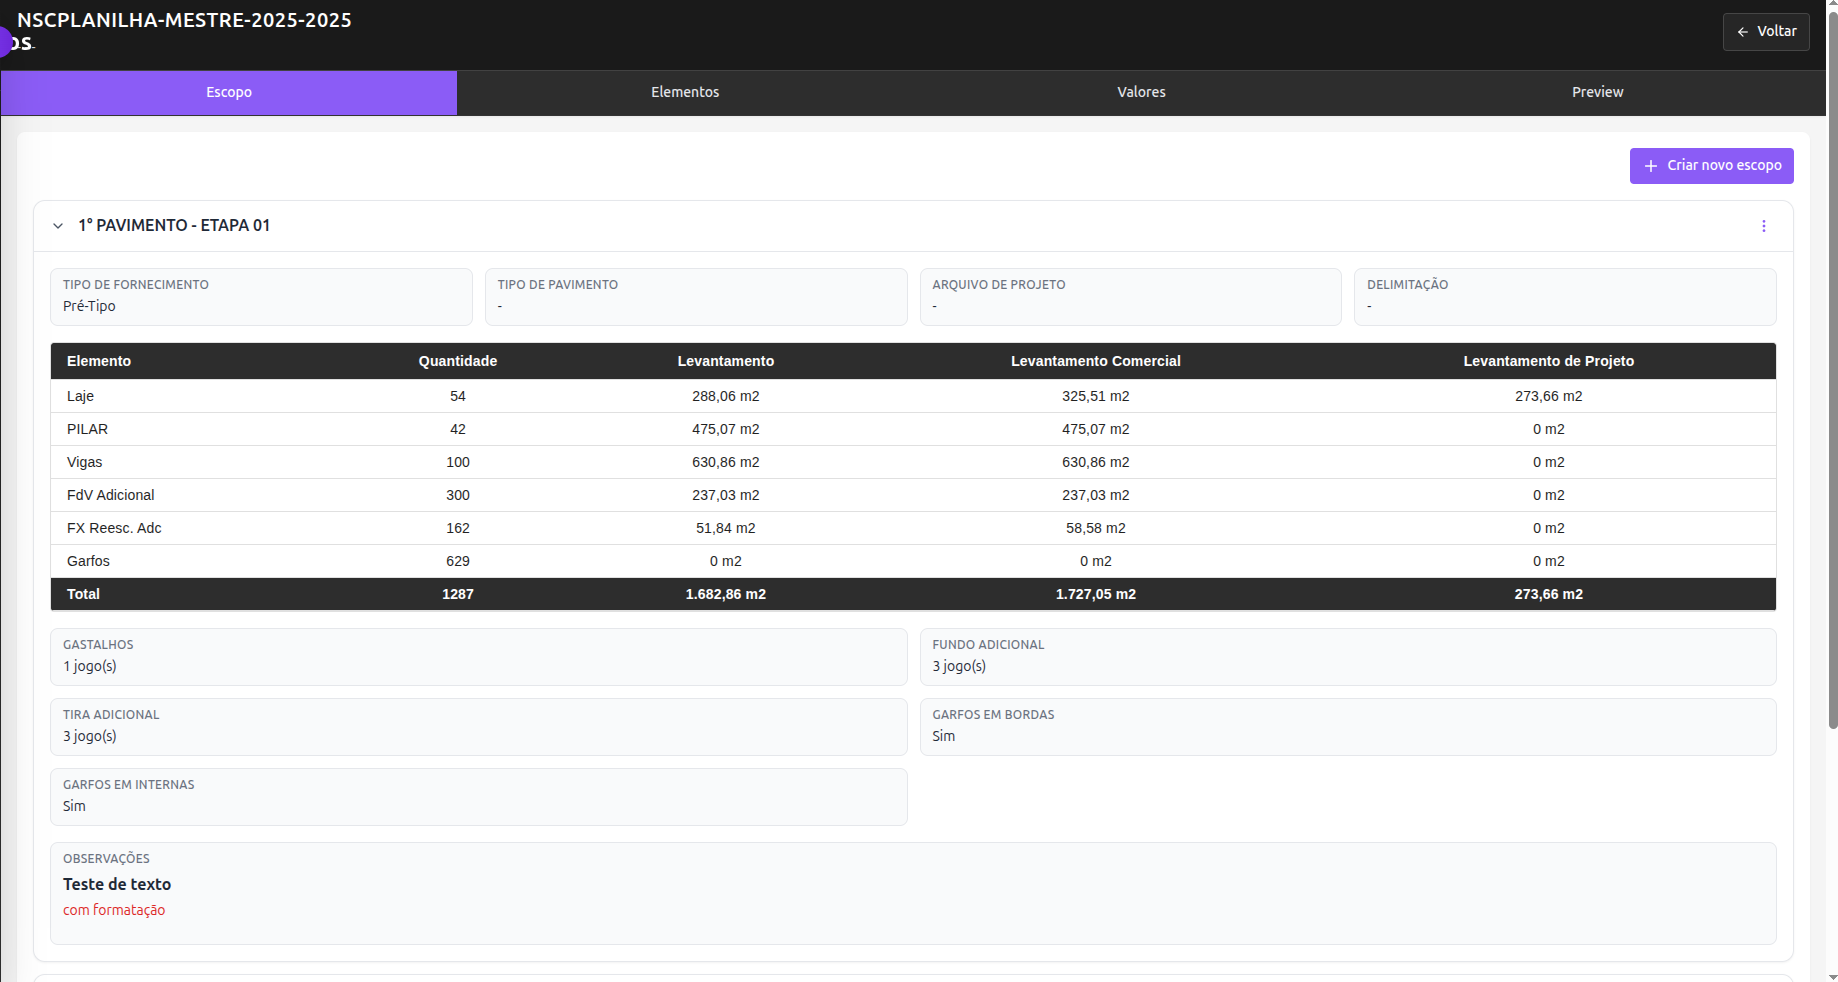
\includegraphics[width=\textwidth]{scope_list.png}
	\legend{Fonte: Elaborado pelos autores, 2026.}
\end{figure}

A \autoref{fig:scope_internal_1} demonstra a primeira parte da página de edição
dos Escopos, que agrupa o gerenciamento dos elementos e a associação de
parâmetros específicos (materiais, custos fixos, taxas de uso).

\begin{figure}[H]
	\caption{\label{fig:scope_internal_1}Interface -- Gerenciamento de Escopo 1}
	\centering
	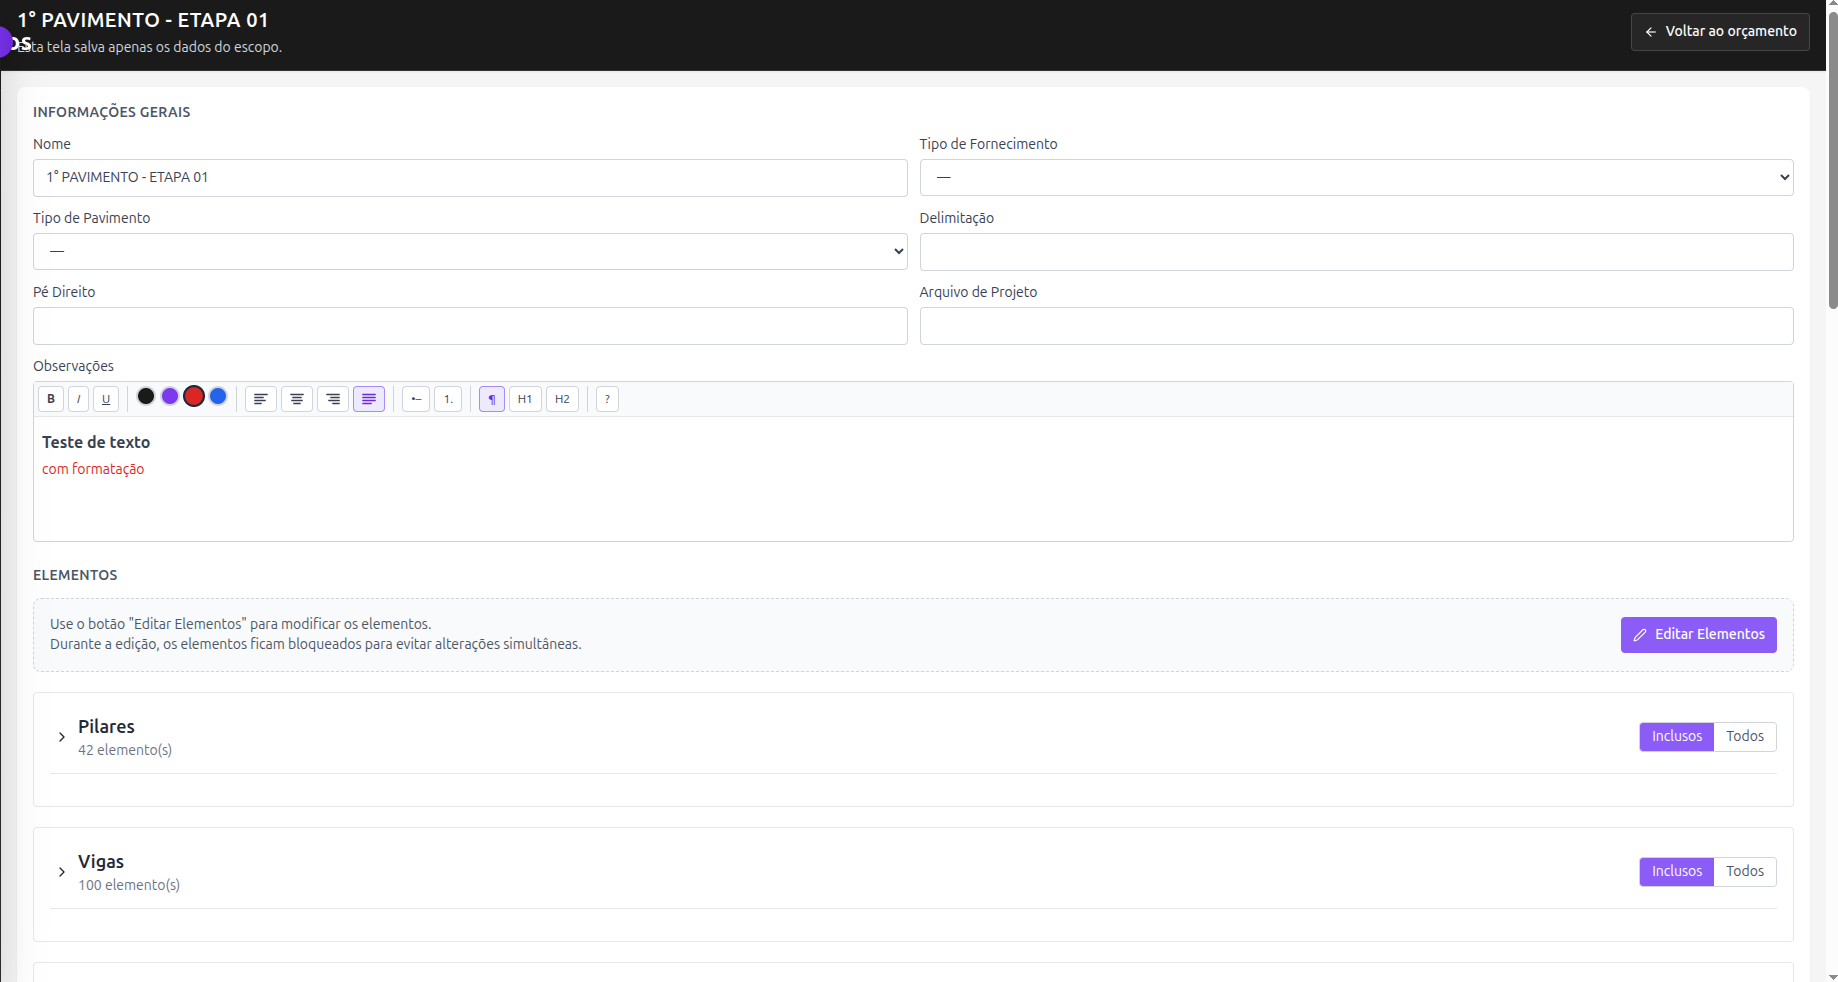
\includegraphics[width=\textwidth]{scope_internal_1.png}
	\legend{Fonte: Elaborado pelos autores, 2026.}
\end{figure}

A \autoref{fig:scope_internal_2} apresenta a continuação dessa página, cujas
configurações são separadas em múltiplas seções e tabelas. Essa separação
limita a quantidade de informação com que o usuário precisa lidar em um
determinado momento, facilitando o uso da aplicação.

\begin{figure}[H]
	\caption{\label{fig:scope_internal_2}Interface -- Gerenciamento de Escopo 2}
	\centering
	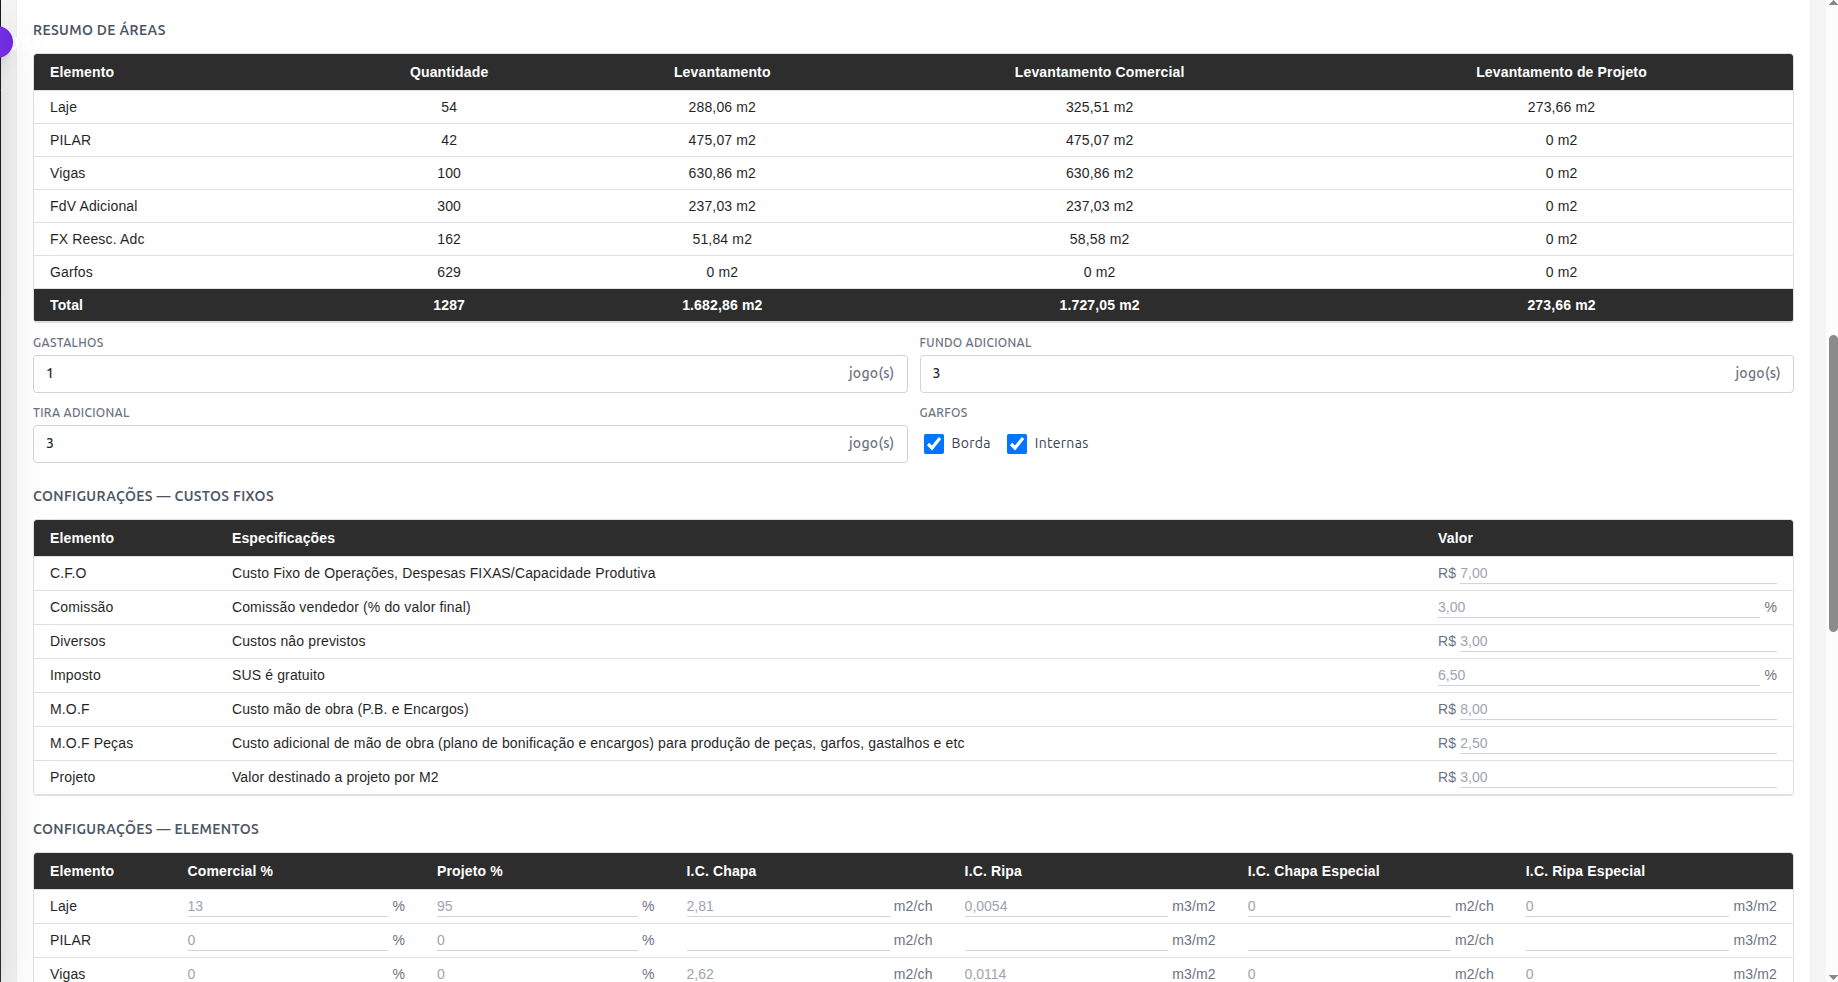
\includegraphics[width=\textwidth]{scope_internal_2.png}
	\legend{Fonte: Elaborado pelos autores, 2026.}
\end{figure}

A \autoref{fig:scope_internal_3} apresenta a parte final da página de edição.
Em todas as suas partes, a utilização de termos e de uma estrutura similares
aos que estavam presentes nas antigas planilhas da empresa aumenta as chances
de uma transição fácil.

\begin{figure}[H]
	\caption{\label{fig:scope_internal_3}Interface -- Gerenciamento de Escopo 3}
	\centering
	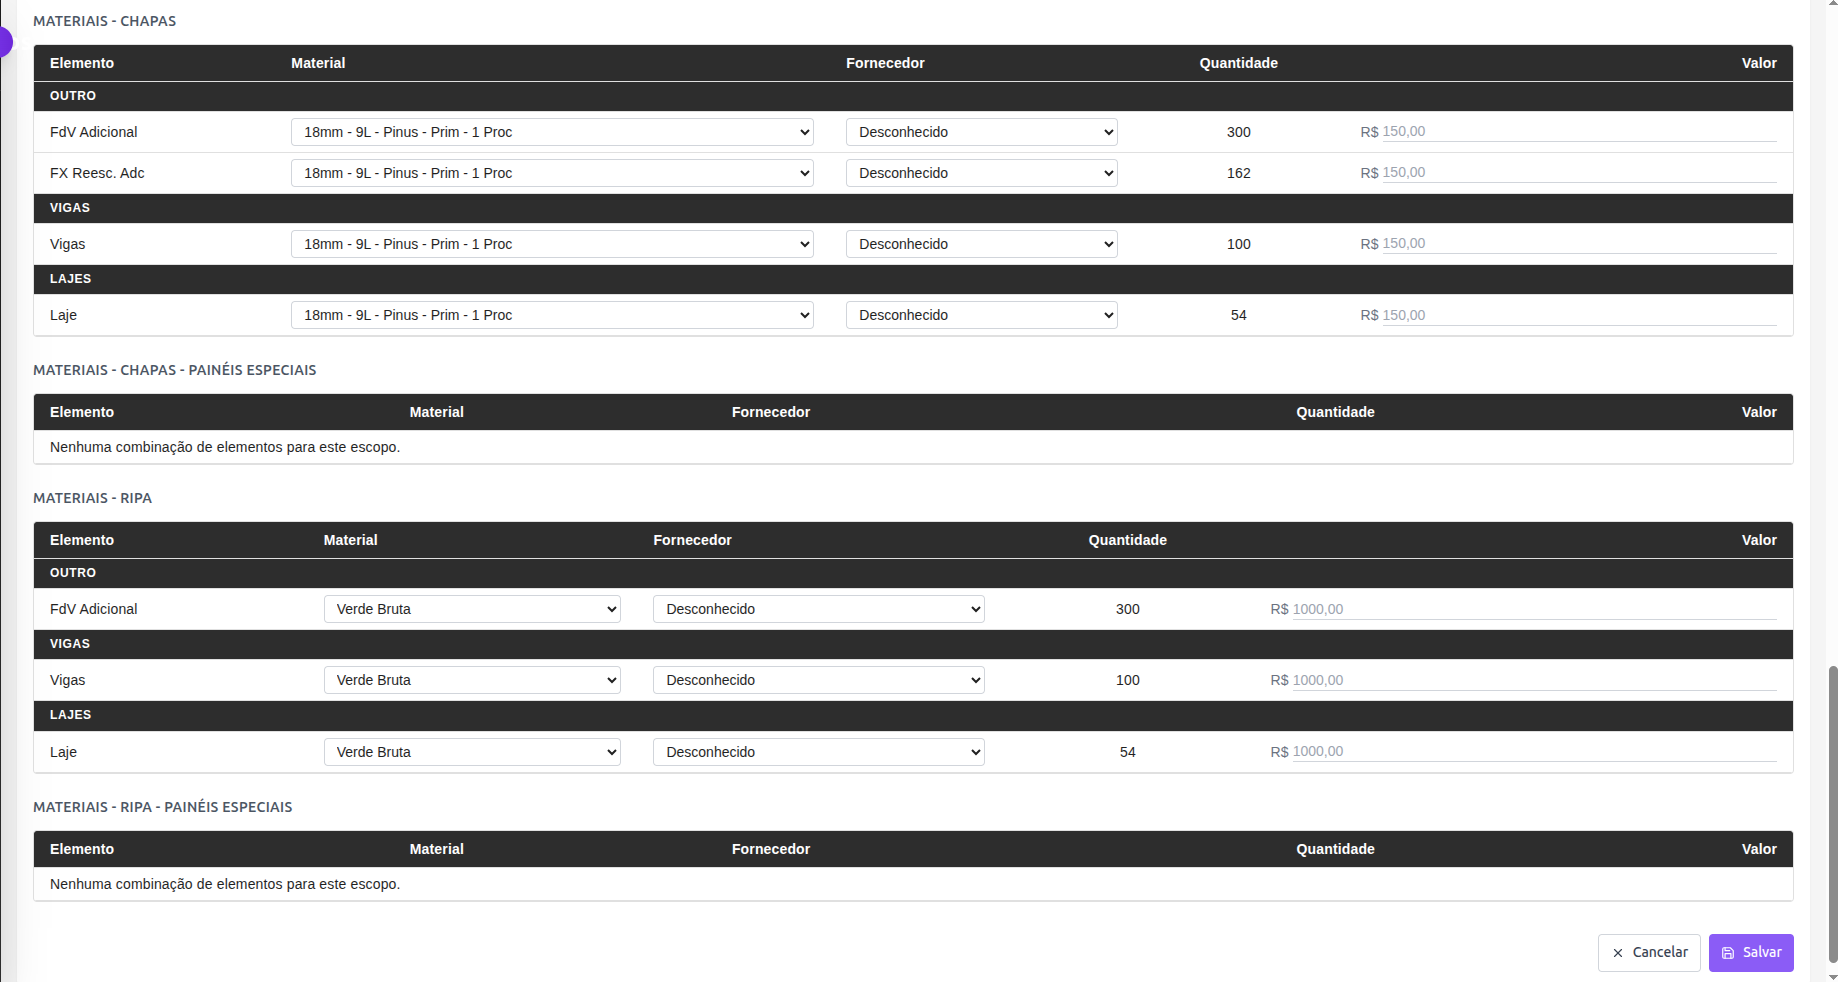
\includegraphics[width=\textwidth]{scope_internal_3.png}
	\legend{Fonte: Elaborado pelos autores, 2026.}
\end{figure}

A aba Valores consolida informações de preços, consumo de materiais e custos
agregados, facilitando a visualização do impacto financeiro de cada decisão.

A \autoref{fig:values_1} demonstra como todas as configurações dos escopos são
agregadas, mostrando os totais de metragem e custo para os materiais.

\begin{figure}[H]
	\caption{\label{fig:values_1}Interface -- Valores -- Agregação de Materiais}
	\centering
	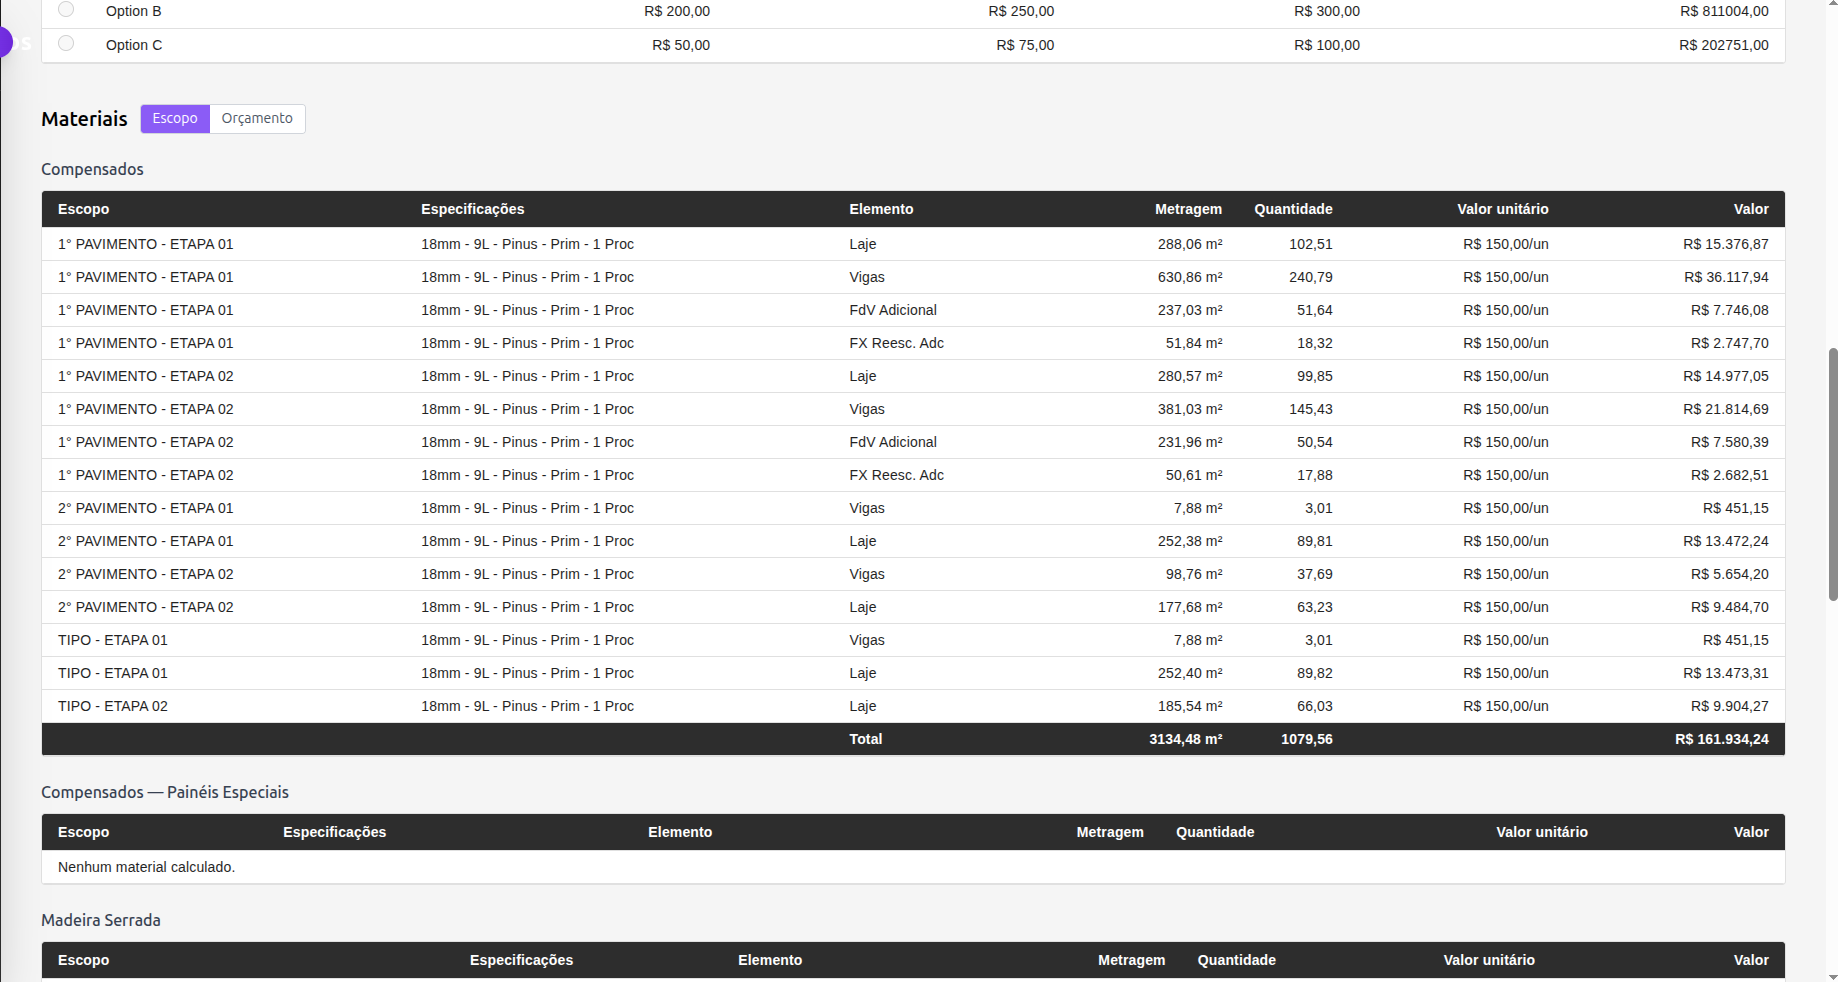
\includegraphics[width=\textwidth]{values_1.png}
	\legend{Fonte: Elaborado pelos autores, 2026.}
\end{figure}

Esses valores são então somados, o resultado servindo ao usuário como uma
referência para a definição do preço a ser cobrado na proposta. A
\autoref{fig:values_2} apresenta as opções de precificação, por meio das quais
esse preço é configurado.

\begin{figure}[H]
	\caption{\label{fig:values_2}Interface -- Valores -- Opções de Precificação}
	\centering
	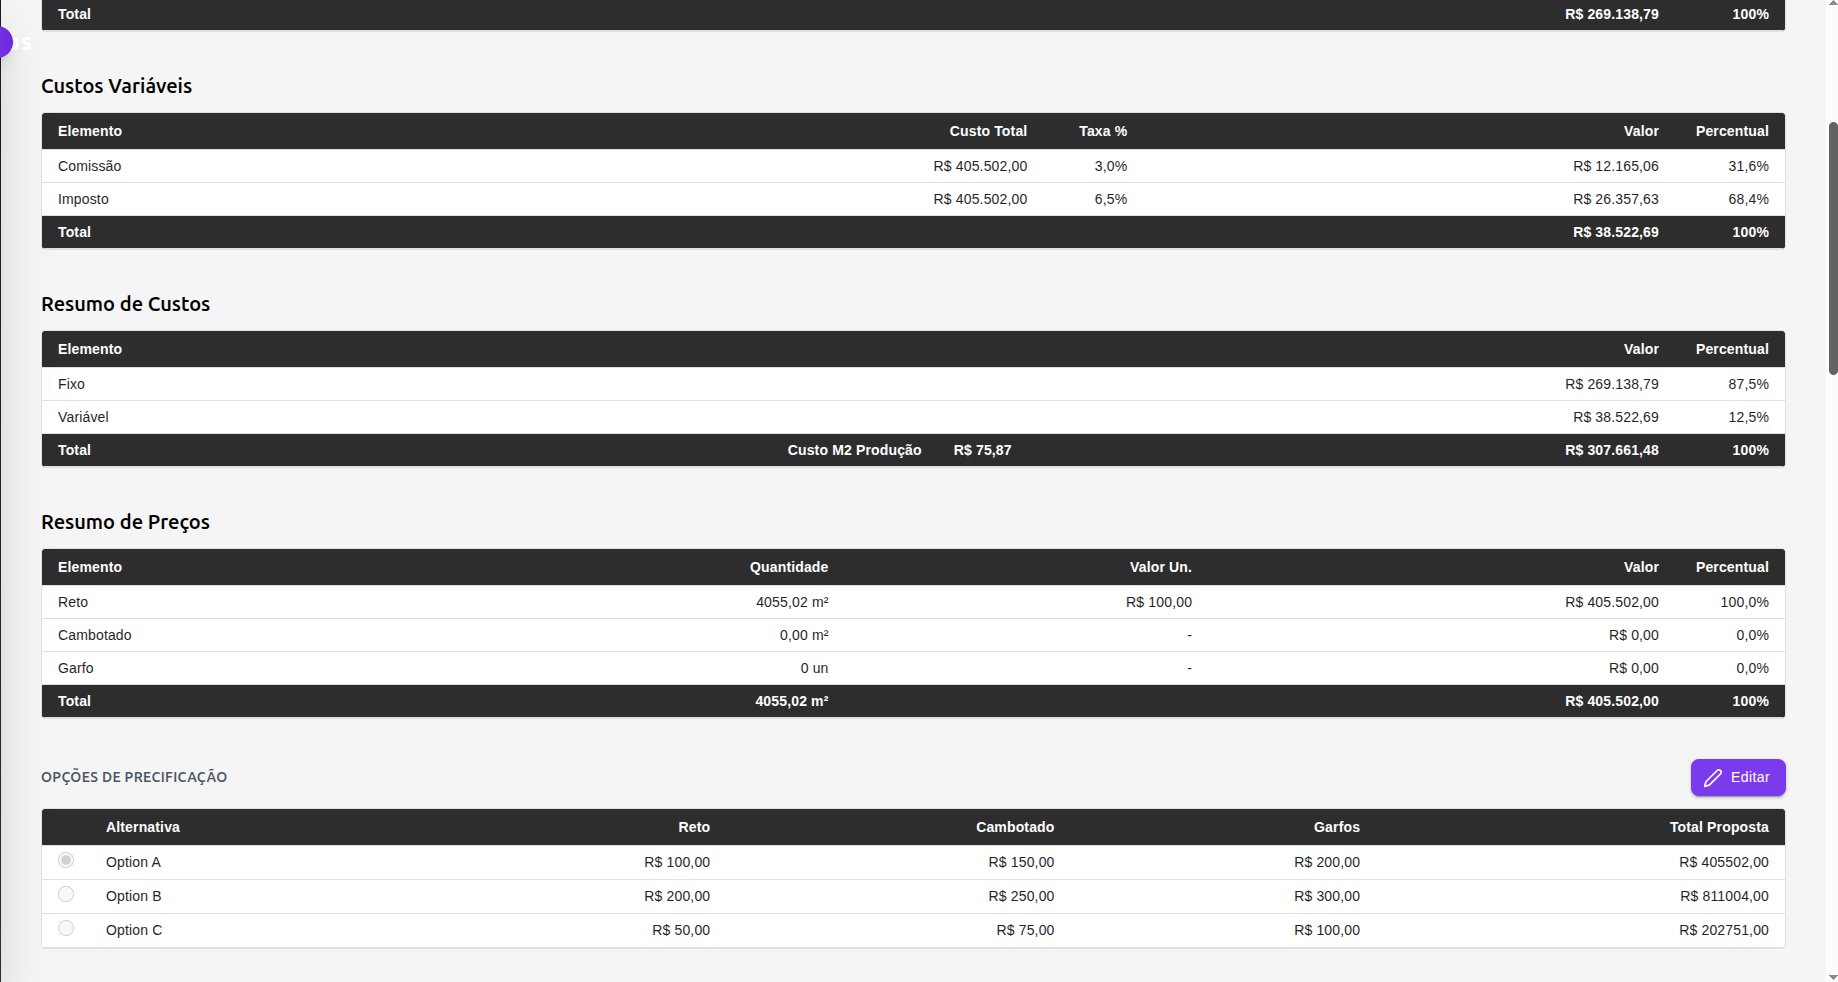
\includegraphics[width=\textwidth]{values_2.png}
	\legend{Fonte: Elaborado pelos autores, 2026.}
\end{figure}

As configurações e inserções de dados são consolidadas na aba \textit{Preview},
que apresenta uma visualização prévia do documento de proposta, permitindo
ajuste de texto e formatação antes da geração final. O sistema também permite
adicionar imagens. A \autoref{fig:export_1} demonstra o sumário do documento.

\begin{figure}[H]
	\caption{\label{fig:export_1}Interface -- Proposta -- Sumário do Documento}
	\centering
	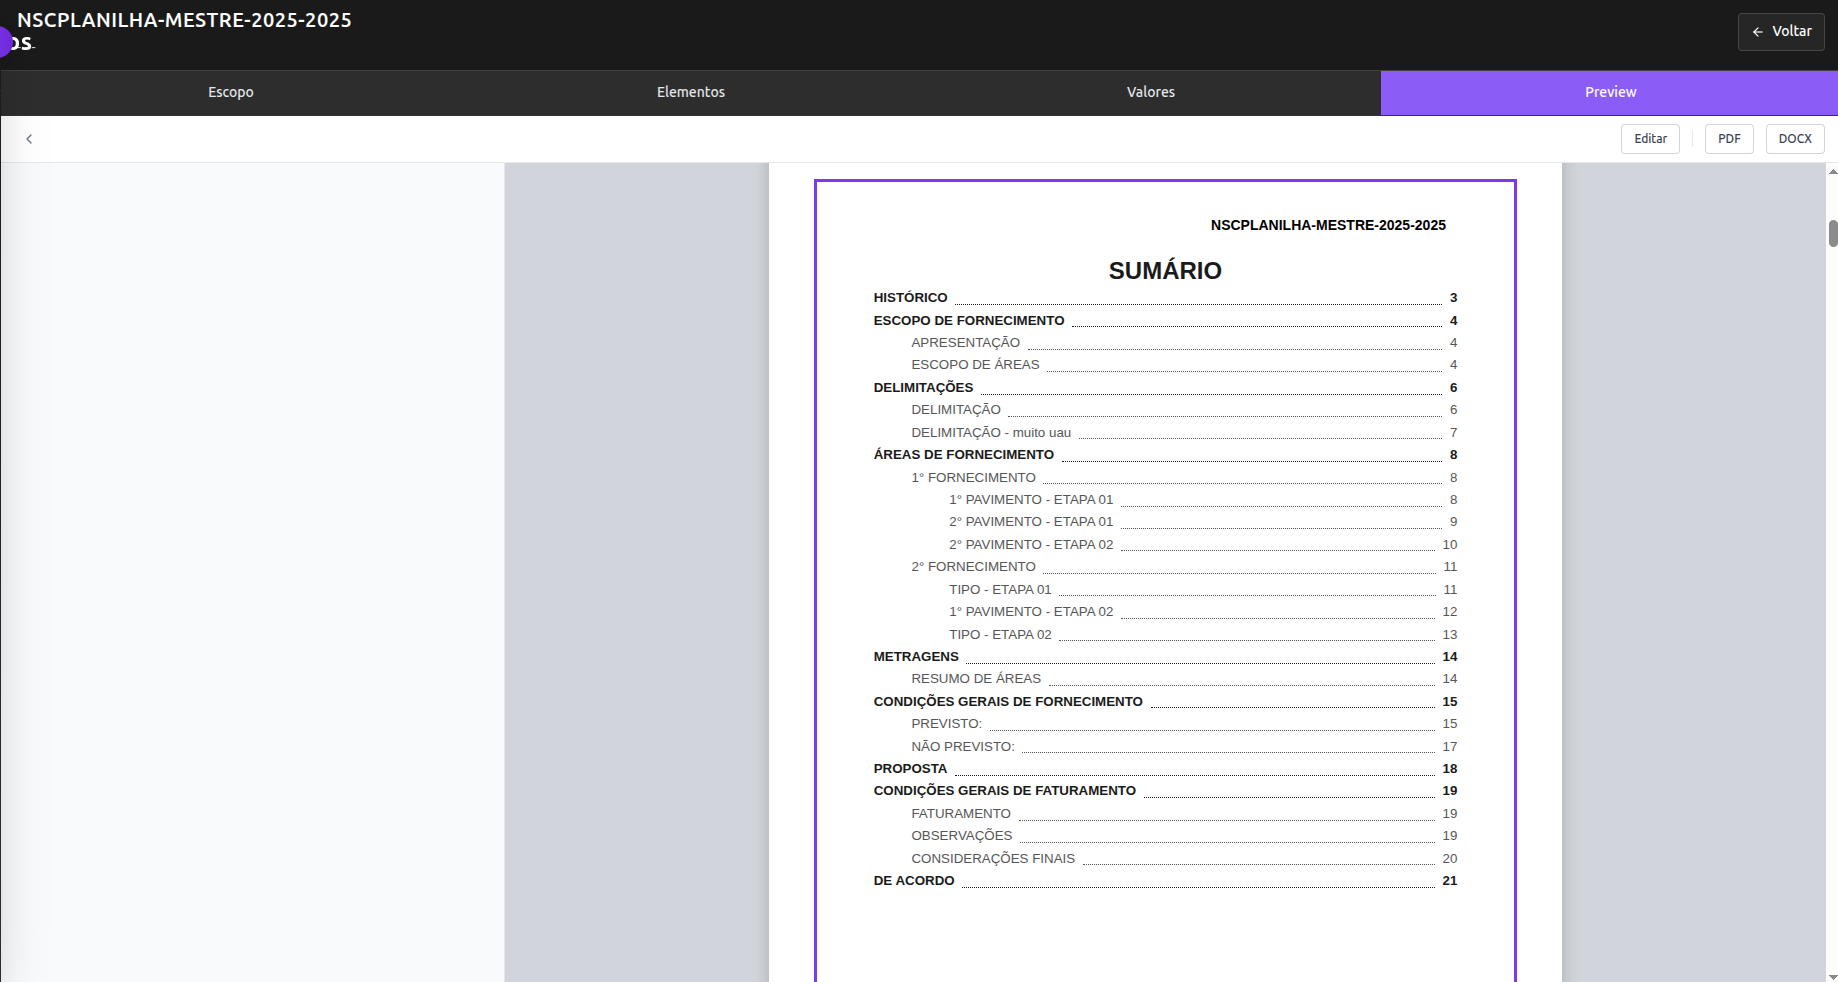
\includegraphics[width=\textwidth]{export_1.png}
	\legend{Fonte: Elaborado pelos autores, 2026.}
\end{figure}

A \autoref{fig:export_2} apresenta as informações de um Escopo, nas quais o
sistema inclui automaticamente o total de metragem.

\begin{figure}[H]
	\caption{\label{fig:export_2}Interface -- Proposta -- Informações de um Escopo}
	\centering
	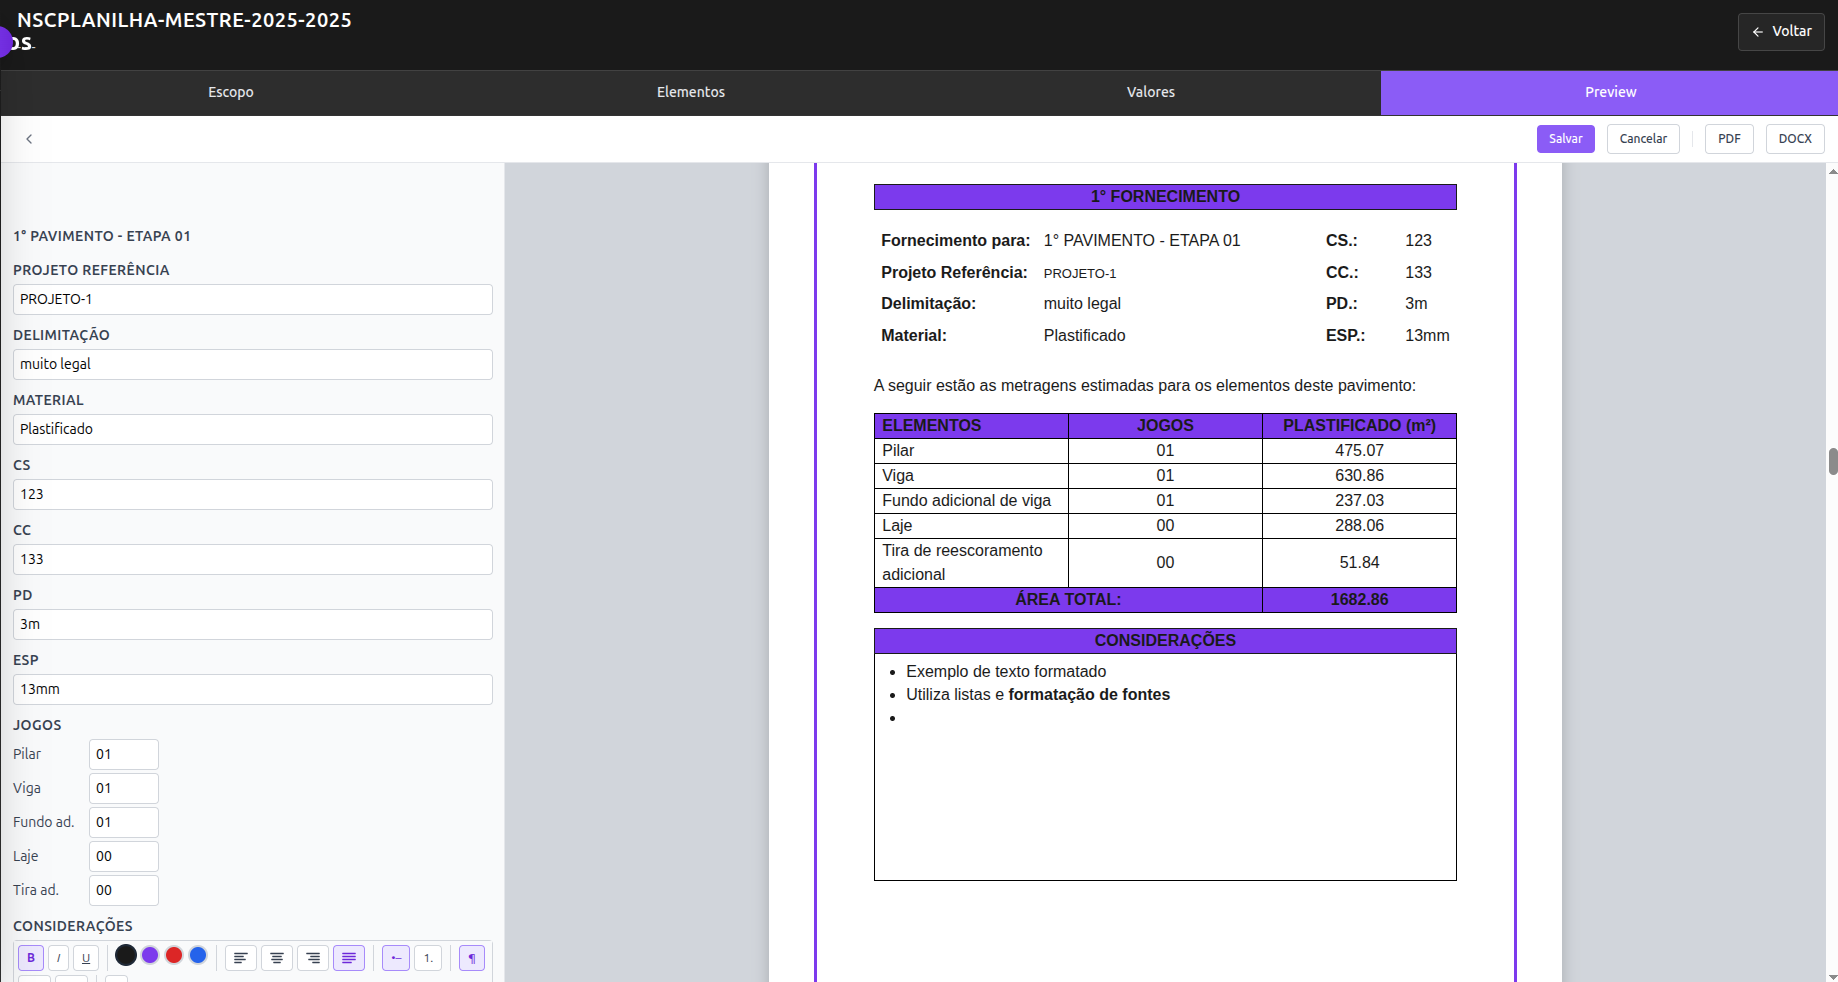
\includegraphics[width=\textwidth]{export_2.png}
	\legend{Fonte: Elaborado pelos autores, 2026.}
\end{figure}

A \autoref{fig:export_3} mostra, por fim, os valores da proposta, que incluem
os preços finais.

\begin{figure}[H]
	\caption{\label{fig:export_3}Interface -- Proposta -- Valores da Proposta}
	\centering
	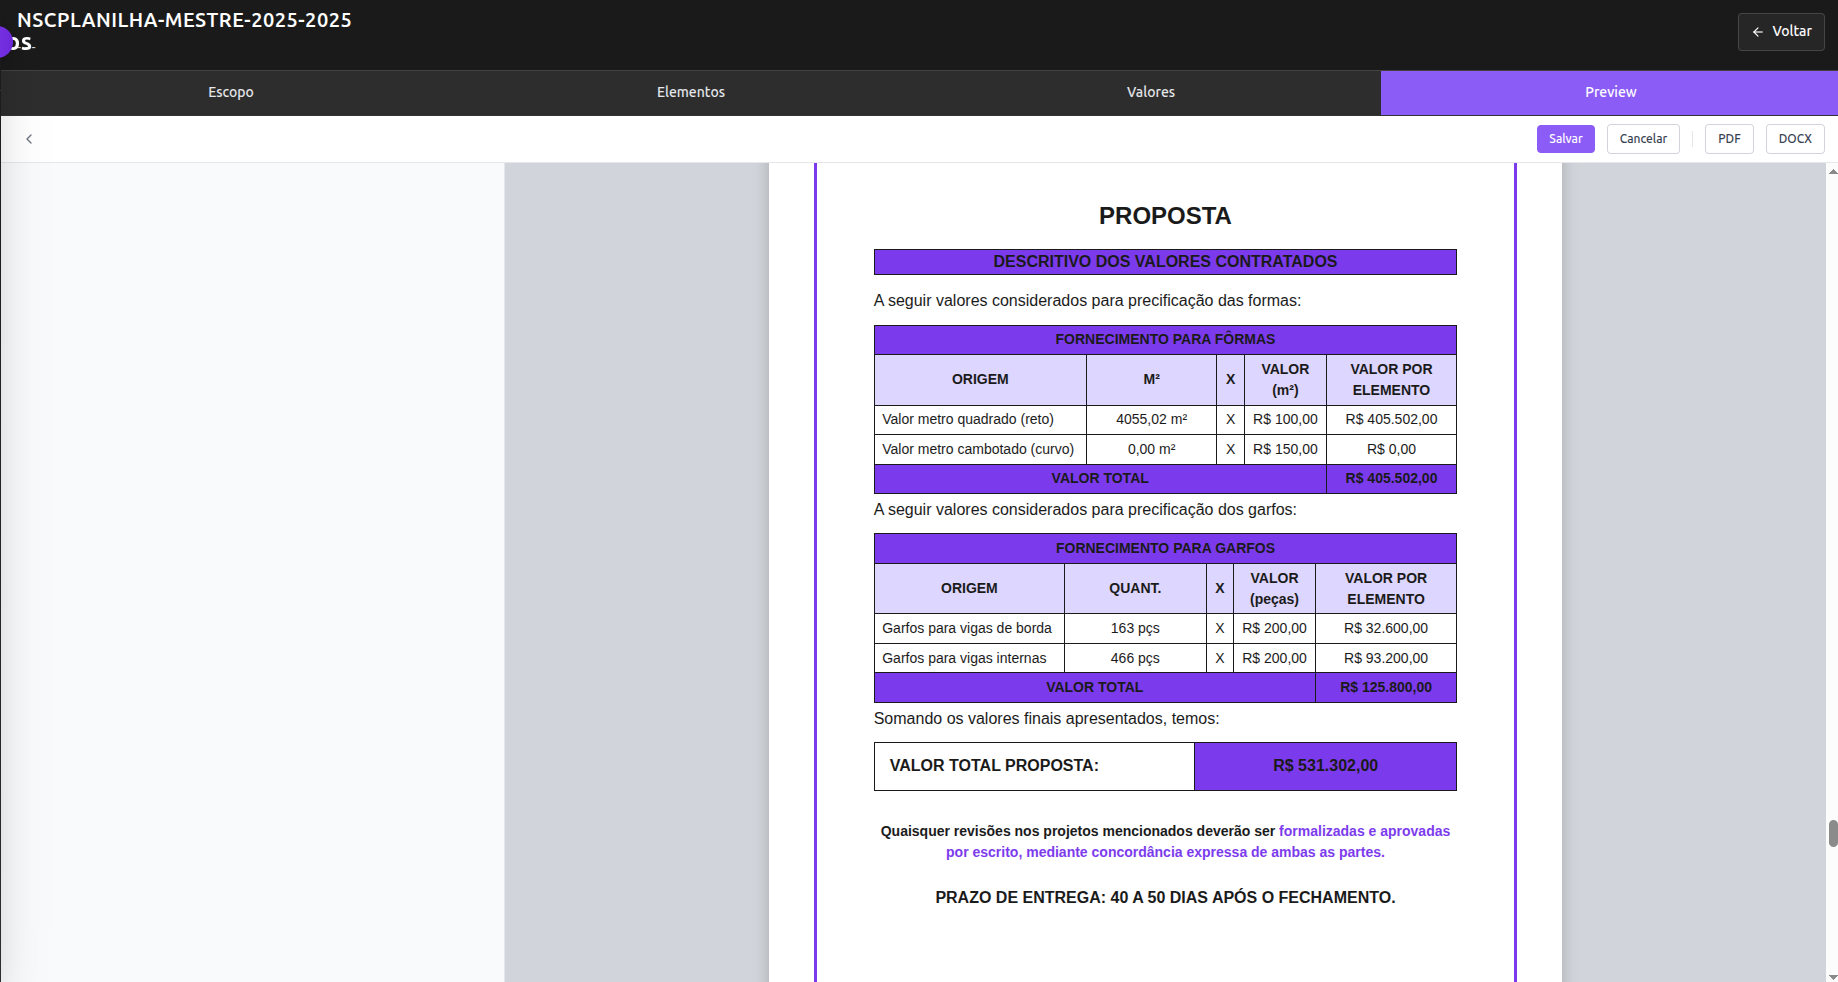
\includegraphics[width=\textwidth]{export_3.png}
	\legend{Fonte: Elaborado pelos autores, 2026.}
\end{figure}

Após a modificação da proposta, as opções de exportação do documento por PDF e
DOCX ficam disponíveis. A primeira realiza a conversão do HTML para o formato
diretamente e a segunda conta com um sistema separado que reconstrói os
elementos no formato de arquivo DOCX, já que uma conversão direta não é
possível.

Cada etapa do fluxo foi desenhada para fornecer sinais claros ao usuário sobre
o estado do documento (bloqueios, alterações pendentes) e para permitir ações
atômicas e reversíveis quando necessário, buscando um produto que preza pela
usabilidade, com o emprego, por exemplo, das dez heurísticas de Nielsen
\cite{nielsen1994}.

Todos os objetivos estabelecidos para o projeto foram atingidos e o trabalho
realizado produziu uma base sólida e funcional para que a implementação de
trabalhos futuros seja realizada.

O mecanismo de coordenação de uso por meio de bloqueio pessimista aplicado por
área de edição foi implementado com sucesso, fornecendo retorno visual na
interface e proteções para evitar bloqueios persistentes em caso de
encerramentos inesperados. Essa funcionalidade poderá ser reutilizada em
implementações futuras. \glossary{Bloqueio Pessimista}{Estratégia de controle
	de concorrência que reserva exclusividade sobre um recurso antes de
	modificá-lo, prevenindo alterações simultâneas por outros usuários.}

A criação de uma biblioteca contendo as regras de domínio e utilitários de
negócio garante consistência entre \textit{frontend} e \textit{backend} e
facilita testes automatizados sobre a lógica de cálculos e transformações de
dados. Ela poderá ser expandida no futuro, servindo como um local estável para
manter as partes mais importantes do sistema, garantindo segurança ao
desenvolvedor. \glossary{Frontend}{Camada de apresentação de um sistema,
	responsável pela interface visual e pela interação direta com o usuário.}
\glossary{Backend}{Camada de lógica e dados de um sistema, responsável pelo
	processamento e armazenamento das informações, sem interação direta com o
	usuário.} \glossary{Modal}{Elemento de interface que exibe conteúdo em
	sobreposição à tela principal, bloqueando a interação com o restante da
	aplicação até ser fechado ou confirmado.}
\section{CONCLUSÃO}

O módulo de orçamento foi concluído, atingindo os objetivos estabelecidos:
centralização de dados, organização do fluxo em unidades de trabalho
controladas com mecanismos de coordenação, mecanismos de gerenciamento de
dados, cálculo de totais e geração do documento final. A arquitetura adotada
demonstrou-se adequada para proporcionar coerência lógica e agilidade de
desenvolvimento.

Os benefícios práticos observados incluem consolidação de processos
anteriormente dispersos, maior segurança em edições colaborativas por meio de
bloqueios coordenados, e preservação de histórico de revisões, além da
automação dos processos. Estes fatores contribuem diretamente para redução de
retrabalho e melhoria da rastreabilidade.

Durante o desenvolvimento, um dos desafios principais identificados foi a
compreensão do contexto do cliente, já que o domínio de orçamentação na empresa
apresenta complexidades que vão além de processos padrão de engenharia.
Compreender plenamente o contexto, as exceções às regras e as necessidades
específicas da operação demandou sessões iterativas com o cliente, enfatizando
a importância de validação contínua.

Para atender às necessidades desse processo, o sistema foi projetado para ser
altamente flexível, permitindo múltiplas exceções. Isso gerou desafios técnicos
na modelagem de dados e lógica de validação. A solução adotada, baseada na
definição de mecanismos de sobrescrita de valores para determinados escopos de
uso, demonstrou ser eficaz, mas gera grande complexidade e compromete a
manutenibilidade do projeto.

A resolução de problemas, tanto de implementação quanto decorrentes de mudanças
solicitadas pelos usuários, é natural e deve ser conduzida de forma contínua.
Quanto a trabalhos futuros, o principal seria a modificação do sistema para
permitir que seja utilizado por mais de uma empresa em um modelo
\textit{multitenant}. \glossary{Multitenant}{Arquitetura de software que
	permite que múltiplos clientes (\textit{tenants}) compartilhem a mesma
	instância de um sistema, mantendo isolamento de dados e configurações entre
	eles.}

% ----------------------------------------------------------
% ELEMENTOS PÓS-TEXTUAIS
% ----------------------------------------------------------
\postextual
% ----------------------------------------------------------

% ----------------------------------------------------------
% Referências bibliográficas
% ----------------------------------------------------------
\clearpage
\bibliographystyle{abntex2-alf}
\bibliography{tcc-references}

% ----------------------------------------------------------
% Glossário
% ----------------------------------------------------------
%
% Consulte o manual da classe abntex2 para orientações sobre o glossário.
%
\clearpage
\printglossary

\end{document}